% Monografia IFG com texto em português formatado com LaTeX
\documentclass[
	% -- Opções da classe memoir --
	oneside,
    %twoside,			% Para impressão em verso e anverso, oposto a oneside
	a4paper,			% Tamanho do papel
	% -- Opções da classe abntex2 -- %
	chapter=TITLE,		% Títulos de capítulos convertidos em letras maiúsculas
	%section=TITLE,		% Títulos de seções convertidos em letras maiúsculas
	%subsection=TITLE,	% Títulos de subseções convertidos em letras maiúsculas
	%subsubsection=TITLE,% Títulos de subsubseções convertidos em letras maiúsculas
	% -- Opções do pacote babel --
	english,			% Idioma adicional para hifenização
	brazil				% O último idioma é o principal do documento
	]{cls/ifg}

% ---
% Pacotes básicos
% ---
\usepackage[T1]{fontenc}		% Seleção de códigos de fonte
\usepackage[utf8]{inputenc}		% Codificação do documento (conversão automática dos acentos)
% --- 		

% ---
% Pacotes adicionais, usados apenas no âmbito do Modelo Canônico do abnteX2
% ---
\usepackage{lipsum}	% Para geração de dummy text
\usepackage{xcolor,graphicx}
% ---

% ---
% Pacotes de citações
% ---
\usepackage[brazilian,hyperpageref]{backref} % Páginas com as citações na bibl
\usepackage[num,abnt-and-type=e, abnt-year-extra-label=yes,abnt-url-package=html, abnt-repeated-author-omit=yes]{abntex2cite} % Citações padrão ABNT
\usepackage{lastpage}
\usepackage{chngcntr}
\counterwithout{figure}{chapter}

% ---
% Configurações do pacote backref
% Usado sem a opção hyperpageref de backref
\renewcommand{\backrefpagesname}{Citado na(s) página(s):~}
% Texto padrão antes do número das páginas
\renewcommand{\backref}{}
% Define os textos da citação
\renewcommand*{\backrefalt}[4]{
	\ifcase #1
		Nenhuma citação no texto.
	\or
		Citado na página #2.
	\else
		Citado #1 vezes nas páginas #2.
	\fi}
% ---

% ---
% Informações de dados para CAPA e FOLHA DE ROSTO
% ---
% AUTOR, TÍTULO E DATA DE DEFESA %
\autor{Yago Luiz dos Santos}
\referenciaautor{Santos, Yago Luiz}

\titulo{SIG Web Luziânia - Sistema de Informação Geográfico Web da Cidade de Luziânia-GO}

\local{Luziânia}
\data{23 de setembro de 2015}
\orientador{Prof. Msc. Henrique Pereira de Freitas Filho}
\instituicao{Instituto Federal de Educação, Ciência e Tecnologia de Goiás}
\curso{Tecnologia em Análise e Desenvolvimento de Sistemas}
\tipotrabalho{Trabalho de Conclusão de Curso}
\preambulo{Trabalho de Conclusão de Curso apresentado à Coordenação do Curso de Tecnologia em Análise e Desenvolvimento de Sistemas do Instituto Federal de Educação, Ciência e Tecnologia de Goiás - Campus Luziânia, como requisito parcial para obtenção do título de Tecnólogo em Tecnologia em Análise e Desenvolvimento de Sistemas.}
% ---

% Alterando o aspecto da cor azul
\definecolor{blue}{RGB}{41,5,195}
% Informações do PDF
% ---
% Configurações de aparência do PDF final

\makeatletter
\hypersetup{
     	%pagebackref=true,
		pdftitle={\@title},
		pdfauthor={\@author},
    	pdfsubject={\imprimirpreambulo},
	    pdfcreator={\@author},
		pdfkeywords={abnt}{latex}{abntex}{abntex2}{trabalho acadêmico},
		colorlinks=true,       		
    	linkcolor=blue,          	% Cor dos links da internet
    	citecolor=blue,        		% Cor dos links da bib
    	filecolor=magenta,      	% Cor dos links do arquivo
		urlcolor=blue,
		bookmarksdepth=4
}
\makeatother
% ---

% ---
% Espaçamentos entre linhas e parágrafos
% ---

% Identa automaticamente o primeiro parágrafo do texto
\usepackage{indentfirst} 
% O tamanho do parágrafo é dado por:
\setlength{\parindent}{1.3cm}

% Controle do espaçamento entre um parágrafo e outro:
\setlength{\parskip}{0.2cm}  % tente também \onelineskip

% ---
% compila o indice
% ---
\makeindex
% ---

% ----
% Início do documento
% ----
\begin{document}

% Seleciona o idioma do documento (conforme pacotes do babel)
%\selectlanguage{english}
\selectlanguage{brazil}

% Retira espaço extra obsoleto entre as frases.
\frenchspacing

% ----------------------------------------------------------
% ELEMENTOS PRÉ-TEXTUAIS
% ----------------------------------------------------------
% \pretextual

% ---
% Capa
% ---
\imprimircapa
% ---

% ---
% Folha de rosto
% (o * indica que haverá a ficha bibliográfica)
% ---
\imprimirfolhaderosto*
% ---

% ---
% Inserir a ficha bibliografica
% ---
%% \begin{fichacatalografica}
%     \includepdf{fig_ficha_catalografica.pdf}
% \end{fichacatalografica}

\begin{fichacatalografica}
	\sffamily
	\vspace*{\fill}					% Posição vertical
	\begin{center}					% Minipage Centralizado
	\fbox{\begin{minipage}[c][8cm]{13.5cm}		% Largura
	\small
	\imprimirautor
	%Sobrenome, Nome do autor
	
	\hspace{0.5cm} \imprimirtitulo  / \imprimirautor. --
	\imprimirlocal, \imprimirdata-
	
	\hspace{0.5cm} \pageref{LastPage} p. : il. (algumas color.) ; 30 cm.\\
	
	\hspace{0.5cm} \imprimirorientadorRotulo~\imprimirorientador\\
	
	\hspace{0.5cm}
	\parbox[t]{\textwidth}{\imprimirtipotrabalho~--~\imprimirinstituicao,
	\imprimirdata.}\\
	
	\hspace{0.5cm}
		1. Palavra-chave1.
		2. Palavra-chave2.
		2. Palavra-chave3.
		I. Orientador.
		II. Universidade xxx.
		III. Faculdade de xxx.
		IV. Título 			
	\end{minipage}}
	\end{center}
\end{fichacatalografica}


% ---
% Inserir errata
% ---
%\begin{errata}
Elemento opcional da \citeonline[4.2.1.2]{NBR14724:2011}. Exemplo:

\vspace{\onelineskip}

FERRIGNO, C. R. A. \textbf{Tratamento de neoplasias ósseas apendiculares com
reimplantação de enxerto ósseo autólogo autoclavado associado ao plasma
rico em plaquetas}: estudo crítico na cirurgia de preservação de membro em
cães. 2011. 128 f. Tese (Livre-Docência) - Faculdade de Medicina Veterinária e
Zootecnia, Universidade de São Paulo, São Paulo, 2011.

\begin{table}[htb]
\center
\footnotesize
\begin{tabular}{|p{1.4cm}|p{1cm}|p{3cm}|p{3cm}|}
  \hline
   \textbf{Folha} & \textbf{Linha}  & \textbf{Onde se lê}  & \textbf{Leia-se}  \\
    \hline
    1 & 10 & auto-conclavo & autoconclavo\\
   \hline
\end{tabular}
\end{table}

\end{errata}

% ---
% Inserir folha de aprovação
% ---
%% \includepdf{folhadeaprovacao_final.pdf}

\begin{folhadeaprovacao}

  \begin{center}
    {\ABNTEXchapterfont\large\imprimirautor}

    \vspace*{\fill}\vspace*{\fill}
    \begin{center}
      \ABNTEXchapterfont\bfseries\Large\imprimirtitulo
    \end{center}
    \vspace*{\fill}

    \hspace{.45\textwidth}
    \begin{minipage}{.5\textwidth}
        \imprimirpreambulo
    \end{minipage}%
    \vspace*{\fill}
   \end{center}

   %Trabalho aprovado. \imprimirlocal, \imprimirdata:

   \assinatura{\textbf{\imprimirorientador} \\ Orientador\\ \imprimirinstituicao}
   \assinatura{\textbf{Prof.ª Dr.ª Maristela Terto de Holanda} \\ Membro da Banca \\ 
   Universidade de Brasília}
   \assinatura{\textbf{ Prof. Me. Daniel Vitor de Lucena} \\ Membro da Banca \\ \imprimirinstituicao}

   \begin{center}
    \vspace*{0.5cm}
    {\large\imprimirlocal}
    \par
    {\large\imprimirdata}
    \vspace*{1cm}
  \end{center}

\end{folhadeaprovacao}


% ---
% Agradecimentos
% ---
\begin{agradecimentos}
Primeiramente a Deus, por sempre está presente em minha vida. A minha família, por toda dedicação e apoio em todos os momentos. Ao Instituto Federal de Goiás e aos professores pela contribuição pessoal e acadêmica. Ao meu grande orientador, professor Henrique Freitas por sua dedicação e profissionalismo.
\end{agradecimentos}


% ---
% RESUMOS
% ---
\setlength{\absparsep}{18pt} % ajusta o espaçamento dos parágrafos do resumo

% resumo em português
\begin{resumo}

\imprimirreferenciaobra

Para gerenciar o grande volume de informações de serviços da cidade de Luziânia, relacionados a educação, lazer saúde e segurança, é necessário a criação de um sistema de informação capaz de organizar e armazenar essas informações, além de realizar o tratamento computacional das informações que indicam localização geográfica. Um Sistema de Informação Geográfico (SIG) é um sistema de informação com a capacidade de armazenar dados alfanuméricos e geográficos. Neste trabalho, é desenvolvido um Sistema de Informação Geográfico Web (SIG Web) a fim de facilitar a organização, gerenciamento e visualização de dados da cidade de Luziânia relacionados aos serviços de educação, lazer, saúde e segurança.

\textbf{Palavras-chave}: Sistema de Informação Geográfico Web; Dados Geográficos; Educação; Lazer; Saúde; Segurança; Luziânia.

\end{resumo} 


% resumo em inglês
\begin{resumo}[Abstract]
 \begin{otherlanguage*}{english}

To manage the large volume information of the city of Luziânia, related to education, entertainment, health and safety, is required an creating information system capable of performing the computational treatment of such information. A Geographic Information System (GIS) is an information system with the ability to store alphanumeric and spatial data. In this paper, was developed a Geographic Information System Web (Web GIS) in order to facilitate the organization, management and visualization of data from city Luziânia related to education, entertainment, health and security.

   \vspace{\onelineskip}

   \noindent
   \textbf{Keywords}: Geographic Information System Web; Geographics Data; Education; Entertainment; Health; Security; Luziânia.
   
 \end{otherlanguage*}
\end{resumo} 


% ---
% inserir lista de ilustrações
% ---
\pdfbookmark[0]{\listfigurename}{lof}
\listoffigures*
\cleardoublepage
% ---

% ---
% inserir lista de tabelas
% ---
\pdfbookmark[0]{\listtablename}{lot}
\listoftables*
\cleardoublepage
% ---

% ---
% inserir o sumario
% ---
\pdfbookmark[0]{\contentsname}{toc}
\tableofcontents*
\cleardoublepage
% ---

% ----------------------------------------------------------
% ELEMENTOS TEXTUAIS
% ----------------------------------------------------------
\textual

\chapter{Introdução}
\label{cap:intro}

\section{Contextualização}

A cidade de Luziânia, município do estado de Goiás, possui uma população de aproximadamente 200 mil habitantes, sendo a quinta maior cidade do Estado \cite{luziania}. Por esse motivo, a cidade possui inúmeras informações sobre serviços básicos que são essenciais para a população, entre eles, serviços relacionados a educação, lazer, saúde e segurança. Atualmente, essas informações são organizadas em documentos físicos e planilhas eletrônicas, o que permite falhas e inconsistências nos dados.

É necessário organizar essas informações de forma a se criar uma base de dados confiável e segura do município, sendo possível inserir novos dados e também novos serviços. Para organizar os dados, será criado um banco de dados utilizando um Sistema Gerenciador de Banco de Dados (SGBD), a fim de facilitar a criação e manutenção dos dados novos e existentes.

Para realizar a visualização dos dados, será desenvolvido um Sistema de Informação Geográfico Web (SIG Web), fazendo uso das tecnologias mais recentes para o desenvolvimento Web. O sistema além de possuir interação em \textit{browsers} a partir de \textit{desktops} e \textit{notebooks}, será totalmente acessível em dispositivos móveis como \textit{smartphones} e \textit{tablets}, tornando o acesso rápido e eficiente independentemente da plataforma acessada.

Nesse contexto, este trabalho vai possuir um banco de dados geográfico para organizar os dados relacionados a educação, lazer, saúde e segurança, além de um SIG Web para visualizar e cadastrar dados obtidos.

\section{Problema}

Atualmente, a cidade de Luziânia não possui um sistema que gerencie serviços básicos relacionados a educação, lazer, saúde e segurança. Todas as informações são organizadas apenas em documentos físicos e planilhas eletrônicas, o que dificulta o acesso posterior, permitindo possíveis falhas e inconsistências que podem ser geradas com o tempo. Além disso, não existe um banco de dados para armazenamento e manutenção dos dados, principalmente os que indicam localização geográfica.

\section{Objetivos}

\subsection{Objetivo Geral}

O desenvolvimento de um SIG Web para a cidade de Luziânia, de forma a facilitar a organização, o gerenciamento e a visualização de dados relacionados aos serviços de educação, lazer, saúde e segurança.

\newpage

\subsection{Objetivos Específicos}

Para atingir o objetivo geral, este trabalho tem como objetivos específicos:

\begin{itemize}
\item Obter dados da cidade de Luziânia relacionados à educação, lazer, saúde e segurança;
\item Especificar o modelo de dados geográfico de acordo com as orientações nacionais;
\item Implementar o banco de dados geográfico em SGBD com extensão espacial;
\item Inserir os dados obtidos no banco de dados geográfico;
\item Desenvolver um SIG Web para a cidade de Luziânia para visualização e cadastro dos dados obtidos;
\item Possuir interação em \textit{browsers} a partir de \textit{desktops} e \textit{notebooks};
\item Ser acessível em dispositivos móveis como \textit{smartphones} e \textit{tablets}.
\end{itemize}

\section{Justificativa}

As informações de serviços básicos da cidade de Luziânia relacionados a educação, lazer, saúde e segurança não são gerenciados através de um sistema para organização e cadastro de novas informações.
Para organizar esses dados, um Sistema de Informação Geográfico (SIG) é fundamental por conseguir armazenar tanto dados alfanuméricos como geográficos. Obtendo assim uma organização mais segura e eficiente, evitando falhas cadastrais de novos dados e permitindo que a população tenha acesso as informações de forma georreferenciada de uma maneira rápida e sem restrições.

\section{Estrutura}

Este trabalho está dividido nos capítulos apresentados a seguir:

\begin{itemize}
\item O Capítulo 2 apresenta os conceitos de Banco de Dados Geográfico;
\item O Capítulo 3 apresenta os conceitos de Sistema de Informação Geográfico;
\item O Capítulo 4 apresenta os resultados obtidos no trabalho;
\item Por último, o Capítulo 5 apresenta as conclusões do trabalho.
\end{itemize}
\chapter{Banco de Dados Geográfico}
\label{cap:bd}

\section{Introdução}

Os bancos de dados geográficos têm como principal característica suportar feições geométricas em suas tabelas, além de oferecer a possibilidade de análise e consultas espaciais. Em outras palavras, esse tipo de banco possibilita a realização de cálculos como áreas e distâncias além de realizar a geração de \textit{buffers} (zona de influência) e outras operações entre as geometrias.

Ao decorrer dos anos, os Sistemas de Informações Geográficos (SIGs) seguiram diferentes formas de implementação, principalmente em relação a estratégia utilizada para armazenar e recuperar dados espaciais. Mais recentemente, os SIGs passaram a utilizar cada vez mais os recursos dos Sistemas Gerenciadores de Banco de Dados (SGBDs), principalmente com o surgimento de extensões espaciais, o que facilitou o desenvolvimento do banco de dados geográfico dos SIGs \cite{gisasp}.

Nas seções deste capítulo, são abordados os principais conceitos relacionados ao paradigma dos quatro universos, modelagem conceitual de dados geográfico, modelo de dados OMT-G, sistema gerenciador de banco de dados, PostGIS e consultas espaciais.

\section{Paradigma dos Quatro Universos}
\label{quatro-universos}

Geoinformação é toda informação passível de espacialização, ou seja, que possua algum tipo de vínculo geográfico que permite sua localização. Este pode ser um ponto, um endereço, um território, entre outros. O problema da geoinformação é a representação computacional do espaço geográfico \cite{harley}.

Para realizar representações computacionais do espaço geográfico, é usado o conceito conhecido como “paradigma dos quatro universos” \cite{velhogomes}. Este paradigma é representado pelo universo ontológico, universo formal, universo estrutural e universo de implementação, como apresentado na Figura \ref{fig:QuatroUniversos}.

\begin{figure}[h]
\centering
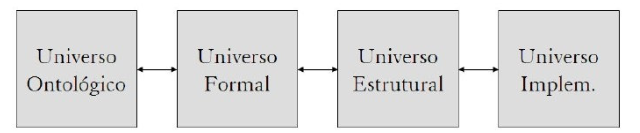
\includegraphics[width=0.65\textwidth]{./img/cap_II/1-QuatroUniversos}
\caption{Paradigma dos quatro universos \cite{queirozferreira}.}
\label{fig:QuatroUniversos}
\end{figure}

A partir do paradigma dos quatro universos, é possível resolver a complexidade que existe entre o mundo real e o mundo computacional.

\subsection{Universo Ontológico}

O universo ontológico inclui os conceitos da realidade a serem modelados no sistema computacional, como os tipos de solo, elementos de cadastro urbano ou rural, dados geofísicos e topográficos.

Um sistema de informação pode ser concebido como um mecanismo de comunicação entre duas partes: o produtor e o usuário. Para que funcione, é necessário que haja uma concordância entre os conceitos das partes. Numa perspectiva mais geral, seu sucesso depende da existência de uma comunidade que compartilhe as definições utilizadas para construí-lo. Para construir um sistema de informação, é preciso definir qual dos diferentes conceitos será representado, como esta representação será construída, e como o usuário pode compreender as características e limitações desta representação. Deste modo, o problema fundamental de um sistema de informação é definir o conjunto de conceitos a ser representado \cite{queirozferreira}.

Para os dados geográficos, uma geo-ontologia é um conjunto de conceitos e um conjunto de relações semânticas e espaciais entre estes termos. Cada conceito tem um nome, uma definição e um conjunto de atributos. O conjunto das relações semânticas inclui as relações de sinonímia, similaridade, e especialização. Os Sistemas de Informações Geográficos (SIGs) e dados geográficos possuem ontologias descritas através do formato \textit{Geographic Markup Language} (GML), proposto pelo consórcio \textit{Open Geospatial Consortium} (OGC) (que será abordado no Capítulo \ref{cap:sig}) \cite{queirozferreira}.

\subsection{Universo Formal}

O universo formal representa um componente intermediário entre os conceitos do universo ontológico e as estruturas de dados e algoritmos computacionais. No universo formal, buscamos estabelecer um conjunto de entidades lógicas que agrupem os diferentes conceitos da ontologia de aplicação da forma mais abrangente possível. O universo formal se divide em duas partes: como medir o mundo real e como generalizar os conceitos da ontologia em entidades formais abrangentes \cite{queirozferreira}.

\subsubsection{Atributos de Dados Geográficos: Teoria da Medida}

Para representar dados geográficos no computador, temos de descrever sua variação no espaço e no tempo. O processo de medida consiste em associar números ou símbolos a diferentes ocorrências de um mesmo atributo, para que a relação dos números ou símbolos reflita as relações entre as ocorrências mensuradas. Por exemplo, podemos medir a poluição do ar em uma cidade em diferentes locais, e cada um desses locais dará um resultado diferente. Esta atribuição é denominada escala de medida \cite{queirozferreira}. Stevens \citeonline{stevens} afirma que há quatro escalas de mensuração: nominal, ordinal, intervalo e razão.

\begin{itemize}
\item A escala nominal classifica objetos em classes distintas sem ordem inerente, como rótulos que podem ser quaisquer símbolos. A Figura \ref{fig:TeoriaMedida} representa a escala nominal.
\item A escala ordinal introduz a idéia de ordenação, caracterizando os objetos em classes distintas que possuem uma ordem natural (por exemplo 1 – ruim, 2 – bom, 3 – ótimo ou “0-10\%”, “11-20\%”, “mais que 20\%”). A Figura \ref{fig:TeoriaMedida} representa a escala ordinal;
\item A escala por intervalo possui um ponto zero arbitrário, uma distância proporcional entre os intervalos e uma faixa de medidas entre [-infinito, +infinito]. A temperatura em graus \textit{Celsius} é um exemplo de medida por intervalo, onde o ponto zero corresponde a uma convenção (a fusão do gelo em água);
\item A escala de razão permite um tratamento mais analítico da informação, pois nela o ponto de referência zero não é arbitrário, mas determinado por alguma condição natural. Sua faixa de valores é limitada entre [0, infinito]. Nesta escala existe um ponto zero absoluto que não pode ser alterado e um intervalo arbitrário com distâncias proporcionais entre os intervalos.
\end{itemize}

\newpage

\begin{figure}[h]
\centering
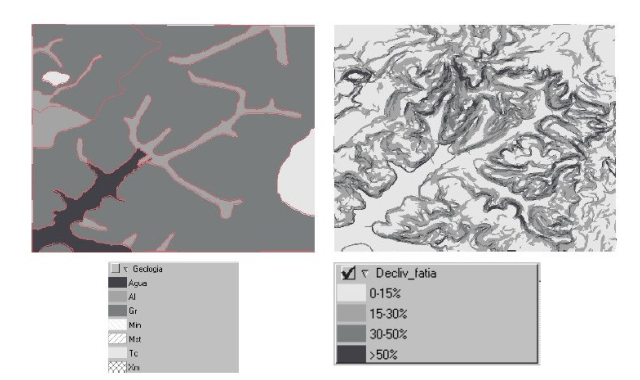
\includegraphics[width=0.75\textwidth]{./img/cap_II/2-TeoriaMedida}
\caption{Exemplo de medida nominal (mapa geológico a esquerda) e medida ordinal (mapa de classes de declividade a direita) \cite{queirozferreira}.}
\label{fig:TeoriaMedida}
\end{figure}

A Tabela \ref{tabela-medidas-geograficas} apresenta um resumo das escalas de medidas, destaca a característica principal, apresenta algumas operações admitidas e exemplos para cada uma delas \cite{queirozferreira}.

\begin{table}[htb]
\IBGEtab{
\caption{Tipo de medidas de dados geográficos \cite{queirozferreira}.}
\label{tabela-medidas-geograficas}
}{
\begin{tabular}{llll}
\toprule
Escala & Características & Exemplos & Operações Possíveis\\
\midrule \midrule
Nominal & Descrição & Tipo de solo, vegetação, uso do solo & Seleção, comparação\\
\midrule
Ordinal & Ordem & Classes de declividade, aptidão de uso & Mediana, máximo, mínimo\\
\midrule
Intervalo & Distância & Altimetria & Diferença, soma\\
\midrule
Razão & Valores absolutos & Renda, população, taxa de natalidade & Operações aritméticas\\
\bottomrule
\end{tabular}}{}
\end{table}

\subsubsection{Espaço Absoluto e Espaço Relativo}

A representação no espaço absoluto se dá através das coordenadas das fronteiras, na Figura \ref{fig:AbsolutoRelativo}, é mostrado a esquerda os distritos da cidade de São Paulo identificados por suas fronteiras. Essa Figura representa o espaço absoluto, pois as fronteiras são estabelecidas na legislação brasileira. E já na imagem da direita, é mostrado um grafo com as conexões dos distritos que formam uma rede, ou seja, a localização exata de cada distrito não é armazenada, pois a rede só captura as relações de adjacência. Essa rede de conexão dos distritos é um modelo de espaço relativo \cite{queirozferreira}.

Para um projeto de um SIG, é fundamental a escolha do tipo de representação que será usado. Esta escolha depende basicamente do tipo de análise a ser realizada pelo sistema. Representações em espaço absoluto são usualmente utilizadas quando as consultas espaciais a serem realizadas envolvem entidades de tipos diferentes. Quando os procedimentos de análise envolvem apenas as relações de conectividade, como, quando se precisa saber o caminho mais curto entre dois distritos \cite{queirozferreira}. Por exemplo, quando se quer saber os municípios vizinhos de uma cidade.

\newpage

\begin{figure}[h]
\centering
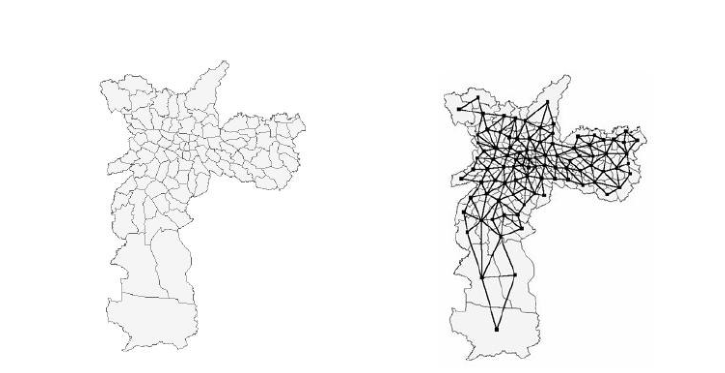
\includegraphics[width=0.75\textwidth]{./img/cap_II/3-AbsolutoRelativo}
\caption{Dualidade entre espaço absoluto e espaço relativo \cite{queirozferreira}.}
\label{fig:AbsolutoRelativo}
\end{figure}

\subsubsection{Modelos no Espaço Absoluto: Geo-Campos e Geo-Objetos}

Existem dois modelos formais para entidades geográficas no espaço absoluto: geo-campos e geo-objetos. O modelo de geo-campos enxerga o espaço geográfico como uma superfície contínua, sobre a qual variam os fenômenos a serem observados. Por exemplo, um mapa de vegetação associa a cada ponto do mapa um tipo específico de cobertura vegetal \cite{queirozferreira}.

O modelo de geo-objetos representa o espaço geográfico como uma coleção de entidades distintas e identificáveis, onde cada entidade é definida por uma fronteira fechada. Por exemplo, um cadastro urbano identifica cada lote como um dado individual, com atributos que o distinguem dos demais \cite{queirozferreira}.

A diferença essencial entre um geo-campo e um geo-objeto é o papel da fronteira, representada na Figura \ref{fig:Geo-CamposObjetos}. A fronteira de um geo-campo é uma divisão arbitrária relacionada apenas com nossa capacidade de medida. Assim, o geo-campo pode ser dividido em partes e ainda assim manter sua propriedade essencial (que é sua função de atributo). Por contraste, um geo-objeto é essencialmente definido por sua fronteira, que o separa do mundo exterior. Ele não pode ser dividido e mantem suas propriedades essenciais. Dentro da fronteira, todas as propriedades do objeto são constantes \cite{queirozferreira}.

\begin{figure}[h]
\centering
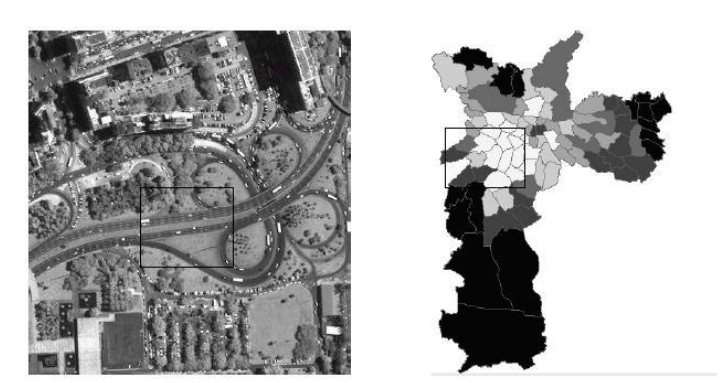
\includegraphics[width=0.75\textwidth]{./img/cap_II/4-Geo-CamposObjetos}
\caption{Exemplo de geo-campo e de geo-objetos \cite{queirozferreira}.}
\label{fig:Geo-CamposObjetos}
\end{figure}

\newpage

\subsubsection{Modelos no Espaço Relativo: Redes}

O modelo de redes concebe o espaço geográfico como um conjunto de pontos no espaço (chamados de nós), conectados por linhas (chamados arcos), onde tanto os nós quanto os arcos possuem atributos. A topologia de redes constitui um grafo onde os recursos que fluem localização geográficas distintas são gravadas \cite{queirozferreira}.

Os fenômenos modelados por redes estão relacionados ao fluxo de pessoas ou materiais, a conexões de influência, a linhas de comunicação e acessibilidade, como por exemplo, na representação dos serviços de utilidade pública, como água, luz e telefone, na representação de rodovias e redes de drenagem (bacias hidrográficas) \cite{harley, queirozferreira}. A Figura \ref{fig:Redes} apresenta um exemplo  do modelo de redes.

\begin{figure}[h]
\centering
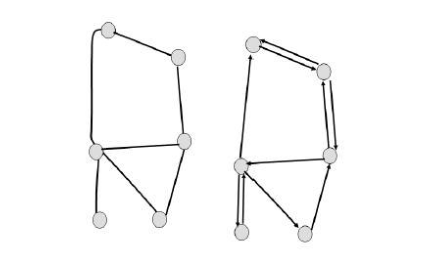
\includegraphics[width=0.50\textwidth]{./img/cap_II/5-Redes}
\caption{Exemplo do modelo de redes \cite{queirozferreira}.}
\label{fig:Redes}
\end{figure}

\subsection{Universo Estrutural}

No universo estrutural as entidades dos modelos formais são mapeadas para estruturas de dados geométricas e alfanuméricas, e algoritmos que realizam operações. As estruturas de dados utilizadas em bancos de dados geográficos podem ser divididas em duas grandes classes: estruturas vetoriais e estruturas matriciais \cite{queirozferreira}. Este trabalho se aprofundará em dados vetoriais, por não ser utilizada nenhuma estrutura matricial para representar algum tipo de dado.

As estruturas vetoriais são utilizadas para representar as coordenadas das fronteiras de cada entidade geográfica, através de três formas básicas: pontos, linhas, e áreas (ou polígonos), definidas por suas coordenadas cartesianas \cite{queirozferreira}. A Figura \ref{fig:EstruturaVetorial} ilustra as estruturas vetoriais.

\begin{figure}[h]
\centering
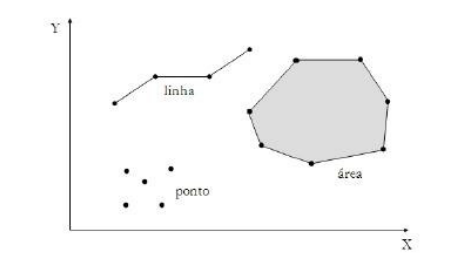
\includegraphics[width=0.55\textwidth]{./img/cap_II/6-EstruturaVetorial}
\caption{Representação das estruturas vetoriais \cite{queirozferreira}.}
\label{fig:EstruturaVetorial}
\end{figure}

\newpage

Um ponto é um par ordenado (x, y) de coordenadas espaciais. O ponto pode ser utilizado para identificar localizações ou ocorrências no espaço. Por exemplo, a localização de crimes, ocorrências de doenças, interseção de cidades. Uma linha é um conjunto de pontos conectados. A linha é utilizada para guardar feições unidimensionais. Por exemplo, um rio que conecta duas cidades distintas. Uma área (ou polígono) é a região do plano limitada por uma ou mais linhas poligonais conectadas de tal forma que o último ponto de uma linha seja idêntico ao primeiro da próxima. Os polígonos são usados para representar unidades de dados geográficos espaciais individuais como por exemplo: distritos, zonas de endereçamento postal e municípios \cite{queirozferreira}.

\subsection{Universo de Implementação}

O quarto e último paradigma contempla o universo de implementação. Neste universo são tomadas todas as decisões para codificação do sistema, como a escolha da arquitetura e a linguagem de programação a ser utilizada.

\section{Modelagem Conceitual de Dados Geográfico}

Um modelo de dados é um agrupamento de conceitos que são usados para descrever as operações e a estrutura em um banco de dados. O modelo busca sistematizar a compreensão a respeito de fenômenos e objetos que serão representados em um sistema informatizado. A modelagem de dados geográficos é bem complexa, pois envolve a discretização do espaço como parte do processo de abstração, visando obter representações adequadas aos fenômenos geográficos \cite{queirozferreira}.

Existe uma grande diferença entre esquema conceitual e modelo de dados conceitual. Esquema conceitual refere-se ao resultado de um conjunto de diagramas que usa um determinado modelo conceitual como uma linguagem para expressar estruturas de dados específicas para uma aplicação, ou seja, se refere ao resultado de uma modelagem. Já um modelo conceitual é uma técnica usada para modelar um banco de dados, incluindo sua notações \cite{queirozferreira}.

Apesar da existência de modelos para a modelagem conceitual como por exemplo, Entidade Relacionamento, \textit{Object Modeling Technique} (OTM) e \textit{Unifed Modeling Language} (UML), esses modelos não atendem as especificidades de dados espaciais. É necessário a aplicação do paradigma dos quatro universos, apresentada na seção \ref{quatro-universos}, para que seja possível agregar dados espaciais em seus modelos.

\subsection{Modelo de Dados OMT–G}
\label{modelo-omtg}

O \textit{Object Modeling Technique for Geographic Applications} (OMT-G) foi elaborado a partir das primitivas definidas do diagrama de classes da UML, adicionando-se primitivas geográficas com o objetivo de aumentar a capacidade de representação semântica do espaço. O modelo OMT-G vem com primitivas para modelar a geometria e topologia dos dados geográficos, oferecendo suporte a estruturas topológicas, estrutura de rede, múltiplas representações de objetos e relacionamentos espaciais, oferecendo também a especificação de atributos alfanuméricos e métodos ligados a cada classe \cite{omtg}.

Existe três conceitos principais para esse modelo: classes, relacionamento e restrições de integridade espaciais. Relacionamento e classes definem as primitivas básicas usadas para criação de esquemas estáticos de aplicação. Além do mais, OMT-G propõe o uso de três diferentes diagramas no processo de desenvolvimento de uma aplicação geográfica: diagrama de classes, diagrama de apresentação e diagrama de transformação, mas destes diagramas, o mais usado é o de classes, visto que ele contém as classes especificadas junto com suas representações e relacionamentos \cite{omtg}.

Por ser o diagrama mais utilizado, a seguir serão apresentadas as definições do modelo OMT-G para criação do diagrama de classes em aplicações geográficas.

\subsubsection{Classes}

Nas aplicações geográficas, encontram-se três grandes grupos de dados: os contínuos, os discretos e os não-espaciais. As classes definidas pelo modelo OMT-G representam esses três grandes grupos. Por meio delas proporcionam uma visão integrada do espaço modelado. Suas classes podem ser georreferenciadas ou convencionais. A distinção entre essas classes permite que aplicações diferentes compartilhem dados não-espaciais, facilitando o desenvolvimento de aplicações integradas e a reutilização de dados \cite{omtg}.

A classe georreferenciada descreve um conjunto de objetos que possuem representação espacial e estão associados a regiões da superfície da terra, representando as visões de geo-campos e geo-objeto (mostradas na seção \ref{quatro-universos} deste trabalho). A classe convencional descreve um conjunto de objetos com propriedades, comportamento, relacionamentos e semânticas semelhantes, e que possuem alguma relação com os objetos espaciais, mas que não possuem propriedades geográficas \cite{omtg}.

A Figura \ref{fig:ClassesOMTG} apresenta a diferença entre as classes convencionais e georreferenciadas. As classes convencionais são simbolizadas sem distinções como na UML e as classes georreferenciadas são simbolizadas no modelo OMT-G de forma semelhante, apresentando um quadrado do lado superior esquerdo designado para indicar a forma geométrica da representação. Os objetos de ambas as classes podem ou não ter atributos não espaciais associados, listados na seção central da representação completa. Operações ou métodos são especificados na seção inferior do retângulo \cite{omtg}.

\begin{figure}[h]
\centering
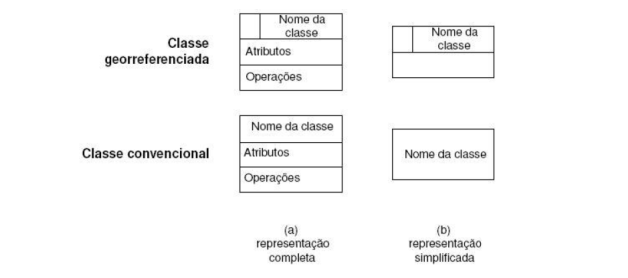
\includegraphics[width=0.70\textwidth]{./img/cap_II/7-ClassesOMTG}
\caption{Classes georreferenciadas e convencionais no OMT-G \cite{omtg}.}
\label{fig:ClassesOMTG}
\end{figure}

O modelo OMT-G apresenta um conjunto fixo de alternativas de representação geométrica, usando uma simbologia que distingue geo-campos e geo-objetos. O modelo OMT-G define cinco classes descendentes de geo-campos: (rede triangular irregular, isolinhas, subdivisão planar, tesselação e amostras) e duas descendentes de geo-objetos: (geo-objetos com geometria e geo-objetos com geometria e topologia). A Figura \ref{fig:ClassesGeo-campos} e a Figura \ref{fig:ClassesGeo-objetos} representam respectivamente as classes descendentes de geo-campos e geo-objetos \cite{omtg}.

\newpage

\begin{figure}[h]
\centering
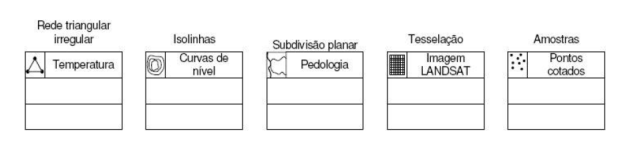
\includegraphics[width=0.70\textwidth]{./img/cap_II/8-ClassesGeo-campos}
\caption{Classes descendentes de geo-campos \cite{omtg}.}
\label{fig:ClassesGeo-campos}
\end{figure}

\begin{figure}[h]
\centering
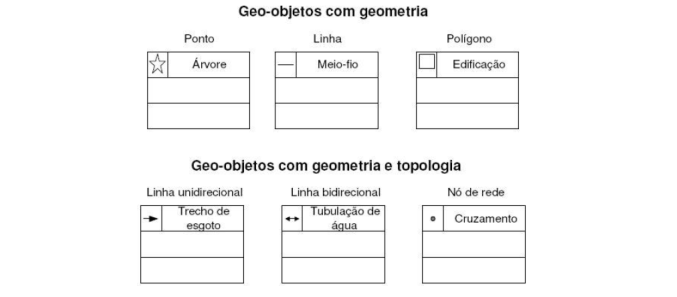
\includegraphics[width=0.70\textwidth]{./img/cap_II/9-ClassesGeo-objetos}
\caption{Classes descendentes de geo-objetos \cite{omtg}.}
\label{fig:ClassesGeo-objetos}
\end{figure}

A classe geo-objeto com geometria representa objetos que possuem apenas propriedades geométricas. Como exemplo, especializada nas classes Ponto, Linha e Polígono, indicando respectivamente, árvore, meio fio e edificação, representados nas classes de geo-objeto com geometria conforme a Figura \ref{fig:ClassesGeo-objetos} \cite{omtg}.

A classe geo-objeto com geometria e topologia representa objetos que possuem além das propriedades geométricas, propriedades de conectividade topológica, sendo especificamente voltadas para a representação de estruturas em rede, como por exemplo, sistemas de abastecimento de água ou fornecimento de energia elétrica. Essas propriedades estão presentes em classes descendentes que representam nós e arcos, da forma usualmente adotada na teoria dos grafos. Os arcos podem ser unidirecionais, como em redes de esgoto, ou bidirecionais, como em redes de telecomunicações. Na Figura \ref{fig:ClassesGeo-objetos} são representados as classes de geo-objeto com geometria e topologia \cite{omtg}.

\subsubsection{Relacionamentos}

Como as relações espaciais e não-espaciais na compreensão do espaço modelado possuem uma enorme importância, o modelo OMT-G representa três tipos de relacionamentos entre suas classes: associação simples, relacionamentos espaciais e relacionamento topológico em rede. Esses três tipos de relacionamentos têm como objetivo definir explicitamente o tipo de interação entre as classes \cite{omtg}.

Associações simples representam relacionamentos estruturais entre objetos de classes diferentes, convencionais ou georreferenciadas. No modelo OMT-G, essas associações são indicadas por linhas contínuas, como mostra a Figura \ref{fig:RelacionamentosOMTG} (a) \cite{omtg}.

Os relacionamentos espaciais representam relações topológicas e métricas. No modelo OMT-G, esse relacionamento é indicado por linhas pontilhadas como mostra a Figura \ref{fig:RelacionamentosOMTG} (b), diferentemente das associações simples, que são linhas contínuas \cite{omtg}.

\newpage

Os relacionamentos de rede são relacionamentos entre objetos que estão conectados uns com os outros. No modelo OMT-G, esses relacionamentos são representados por duas linhas pontilhadas paralelas como mostra na Figura \ref{fig:RelacionamentosOMTG} (c). Os relacionamentos são geralmente especificados entre classes de nós e uma classe de arcos. No entanto, estruturas de redes sem nós podem ser definidas, especificando um relacionamento recursivo sobre uma classe de arcos, como na Figura \ref{fig:RelacionamentosOMTG} (d) \cite{omtg}.

\begin{figure}[h]
\centering
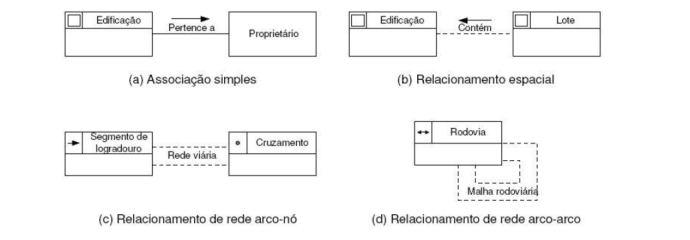
\includegraphics[width=0.80\textwidth]{./img/cap_II/10-RelacionamentosOMTG}
\caption{Relacionamentos no OMT-G \cite{omtg}.}
\label{fig:RelacionamentosOMTG}
\end{figure}

As representações de cardinalidade, generalização e especificação no modelo OMT-G seguem o mesmo padrão da diagramação UML.

\section{Sistema Gerenciador de Banco de Dados}

Um Sistema Gerenciador de Banco de Dados (SGBD) é um sistema de software que possibilita aos usuários criar e manter um banco de dados, facilitando os seguintes processos: definição, construção, manipulação e compartilhamento \cite{bancodados}.

\begin{itemize}
\item A definição de um banco de dados consiste na especificação das estruturas, dos tipos de dados e das restrições para os dados a serem armazenados no banco de dados;
\item A construção de um banco de dados é o armazenamento dos dados em alguma mídia adequada controlada pelo SGBD;
\item A manipulação ocorre a partir de um conjunto de funções, entre essas funções temos as pesquisas em banco de dados que recuperam dados especificados pelo usuário e a atualização do banco que repete as mudanças dos requisitos do banco;
\item O compartilhamento consiste no acesso concorrente ao banco de dados por múltiplos usuários e programas.
\end{itemize}

Os requisitos mais importantes para os Sistemas Gerenciadores de Banco de Dados (SGBDs) são a facilidade de uso, correção, facilidade de manutenção, confiabilidade, segurança e desempenho. Na Tabela \ref{tabela-requisitos-SGBDs} é apresentada a definição de cada requisito e a Tabela \ref{tabela-tecnologias-SGBDs} apresenta as principais tecnologias para os SGBDs a fim de cumprir esses requisitos \cite{queirozferreira}.

\newpage

\begin{table}[htbp]
\IBGEtab{
\caption{Principais requisitos para SGBDs \cite{queirozferreira, bancodados}.}
\label{tabela-requisitos-SGBDs}
}{
\begin{tabular}{ll}
\toprule
Requisito & Definição\\
\midrule \midrule
Facilidade de Uso & A modelagem do banco de dados deve refletir a realidade das aplicações e o acesso aos\\
& dados deve ser feito de forma simples\\
\midrule
Correção & Os dados armazenados no banco de dados devem refletir um estado correto\\
& da realidade modelada\\
\midrule
Facilidade de Manutenção & Alterações na forma de armazenamento dos dados devem afetar as aplicações\\
& o mínimo possível\\
\midrule
Confiabilidade & Atualizações não devem ser perdidas e não devem interferir umas com as outras\\
\midrule
Segurança & O acesso aos dados deve ser controlado de acordo com os direitos definidos para cada\\
& aplicação ou usuário\\
\midrule
Desempenho & O tempo de acesso aos dados deve ser compatível com a complexidade da consulta\\
\bottomrule
\end{tabular}}{}
\end{table}

\begin{table}[htb]
\IBGEtab{
\caption{Principais tecnologias para SGBDs \cite{queirozferreira, bancodados}.}
\label{tabela-tecnologias-SGBDs}
}{
\begin{tabular}{ll}
\toprule
Requisito & Definição\\
\midrule \midrule
Facilidade de Uso & Linguagem de definição de dados, linguagem de consulta baseada em modelo\\
& de dados de alto nível e o fornecimento de múltiplas interfaces para os usuários\\
\midrule
Correção & Restrições de integridade, \textit{triggers} e assertivas\\
\midrule
Facilidade de Manutenção & Especificações do banco de dados em níveis isolando os detalhes\\
& de armazenamento das aplicações\\
\midrule
Confiabilidade & Transações atômicas implementadas através de mecanismos para controle\\
& de concorrência, mecanismos de \textit{backup}, controle de redundância de dados e mecanismos\\
& de recuperação a caso de falhas\\
\midrule
Segurança & Níveis de autorização e controle de acesso\\
\midrule
Desempenho & Otimização de consultas, baseada em métodos de acesso e de armazenamento eficientes,\\
& gerência eficaz do \textit{buffer pool} e modelos de custo, entre outras tecnologias\\
\bottomrule
\end{tabular}}{}
\end{table}

O mercado para SGBDs concentra-se principalmente em duas tecnologias: Os SGBDs Relacionais (SGBD-R) e os SGBDs Objeto-Relacionais (SGBD-OR)\cite{queirozferreira}.

Os SGBD-R seguem o modelo relacional de dados, em que um banco de dados é organizado como uma coleção de relações, cada qual com atributos de um tipo específico. Nos sistemas comerciais atuais, os tipos incluem números inteiros, de ponto flutuante, cadeias de caracteres, datas e campos binários longos (BLOBs). Os SGBD-OR estendem o modelo relacional, entre outras características, com um sistema de tipos de dados rico e estendível, oferecendo operadores que podem ser utilizados na linguagem de consulta \cite{queirozferreira}.

Os SGBD-R foram concebidos para atender as necessidades de aplicações manipulando grandes volumes de dados convencionais. De fato, tais sistemas não oferecem recursos para atender as necessidades de aplicações não convencionais. A mera simulação de tipos de dados não convencionais em um SGBD-R pode ter efeitos colaterais, como queda de desempenho, dificuldade de codificação e posterior manutenção da aplicação. Os SGBD-OR possibilitam a extensão dos mecanismos de indexação sobre os novos tipos. Essas características reduzem os problemas ocorridos na simulação de tipos de dados pelos SGBD-R, tornando os SGBD-OR uma solução atrativa para aplicações não convencionais \cite{queirozferreira}.

Para atender as necessidades dos SIGs, surgiram SGBD-ORs com extensões geográficas \textit{open sources} como o PostGIS. No tópico seguinte, será abordado um pouco mais sobre o PostGIS.

\newpage

\section{PostGIS}

O PostGIS é uma extensão geográfica do SGBD-OR PostgreSQL desenvolvido pela empresa canadense \textit{Refractions Research}, o seu código fonte é aberto através da licença \textit{GNU PLS} \cite{PostGIS}. A Figura \ref{fig:DadosPostGIS} apresenta os tipos de dados espaciais fornecidos por essa extensão. As representações textuais desses tipos são \cite{queirozferreira}:

\begin{itemize}
\item \textit{Point: (0, 0, 0)}
\item \textit{LineString: (0 0, 1 1, 2 2)}
\item \textit{Polygon: ((0 0 0, 4 0 0, 4 4 0, 0 4 0, 0 0 0), (100, ...), ...)}
\item \textit{MultiPoint: (0 0 0, 4 4 0)}
\item \textit{MultiLineString: ((0 0 0, 1 1 0, 2 2 0), (4 4 0, 5 5 0, 6 6 0))}
\item \textit{MultiPolygon: (((0 0 0, 4 0 0 , 4 4 0, 0 4 0, 0 0 0), (...), ...), ...)}
\item \textit{GeometryCollection: (POINT(2 2 0), LINESTRING(4 4 0, 9 9 0))}
\end{itemize}

\begin{figure}[h]
\centering
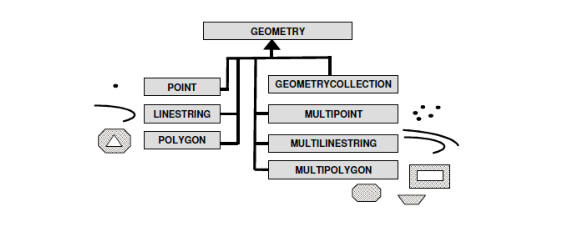
\includegraphics[width=0.70\textwidth]{./img/cap_II/11-DadosPostGIS}
\caption{Tipo de dados espaciais no PostGIS \cite{queirozferreira}.}
\label{fig:DadosPostGIS}
\end{figure}

A Figura \ref{fig:CreatePostGIS} apresenta a criação de uma tabela no PostGIS, que é realizada em duas etapas: na primeira etapa definimos os atributos básicos (alfanuméricos) e na segunda, usamos uma função para adicionar a coluna com o tipo espacial \cite{queirozferreira}.

Utilizamos a função \textit{AddGeometryColumn} para adicionar a coluna com o tipo espacial. Os parâmetros dessa função são \cite{queirozferreira}:

\begin{itemize}
\item Nome do banco de dados;
\item Nome da tabela que irá conter a coluna espacial;
\item Nome da coluna espacial;
\item Sistema de coordenadas em que se encontram as geometrias da tabela;
\item Tipo da coluna espacial, que serve para criar uma restrição que verifica o tipo do objeto sendo inserido na tabela;
\item Dimensão em que se encontram as coordenadas dos dados.
\end{itemize}

\begin{figure}[h]
\centering
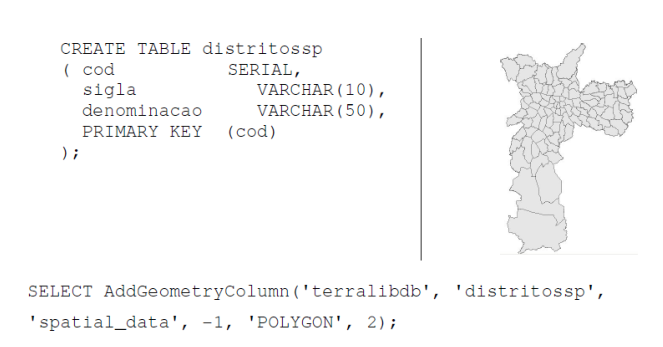
\includegraphics[width=0.70\textwidth]{./img/cap_II/12-CreatePostGIS}
\caption{Criação de uma tabela no PostGIS, adaptado de \cite{queirozferreira}.}
\label{fig:CreatePostGIS}
\end{figure}

Para inserir informações na tabela, utilizamos o comando \textit{SQL INSERT} após a criação das tabelas de dados. Para inserção da geometria, utilizamos a representação textual das geometrias em conjunto com a função \textit{GeometryFromText} que recebe a representação textual mais o sistema de coordenadas em que se encontra a geometria, apresentada na Figura \ref{fig:InsertPostGIS} \cite{queirozferreira}.

\begin{figure}[h]
\centering
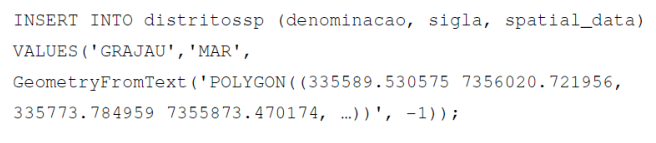
\includegraphics[width=0.70\textwidth]{./img/cap_II/13-InsertPostGIS}
\caption{Inserindo informações em uma tabela, adaptado de \cite{queirozferreira}.}
\label{fig:InsertPostGIS}
\end{figure}

A Figura \ref{fig:SelectPostGIS} apresenta um exemplo de recuperação de informações de uma tabela. O comando seleciona a linha do bairro “Vila Mariana” e utiliza a função \textit{AsText} para obter como resultado a geometria associada ao bairro de forma textual \cite{queirozferreira}.

\begin{figure}[h]
\centering
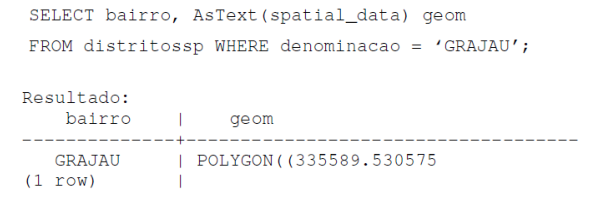
\includegraphics[width=0.70\textwidth]{./img/cap_II/14-SelectPostGIS}
\caption{Recuperando informações de uma tabela, adaptado de \cite{queirozferreira}.}
\label{fig:SelectPostGIS}
\end{figure}

\newpage

Na Figura \ref{fig:IndexPostGIS}, é apresentada a sintaxe básica para a criação de uma indexação espacial e um exemplo de criação em uma tabela \cite{queirozferreira}.

\begin{figure}[h]
\centering
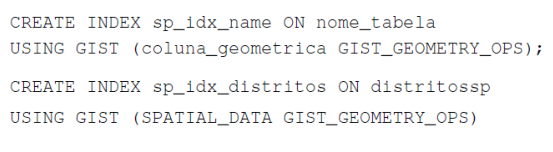
\includegraphics[width=0.70\textwidth]{./img/cap_II/15-IndexPostGIS}
\caption{Indexação espacial, adaptado de \cite{queirozferreira}.}
\label{fig:IndexPostGIS}
\end{figure}

Os índices espaciais são usados em consultas que envolvem predicados espaciais, como no caso de consultas por janela, no qual um retângulo é informado e as geometrias que interagem com ele devem ser recuperadas rapidamente.

\section{Consultas Espaciais}

O PostGIS possui vários operadores espaciais disponíveis que são fornecidos através da integração do PostGIS com a biblioteca \textit{Geometry Engine Open Source} (GEOS). A Figura \ref{fig:OperadoresPostGIS} mostra uma relação de vários operadores disponíveis \cite{queirozferreira}.

\begin{figure}[h]
\centering
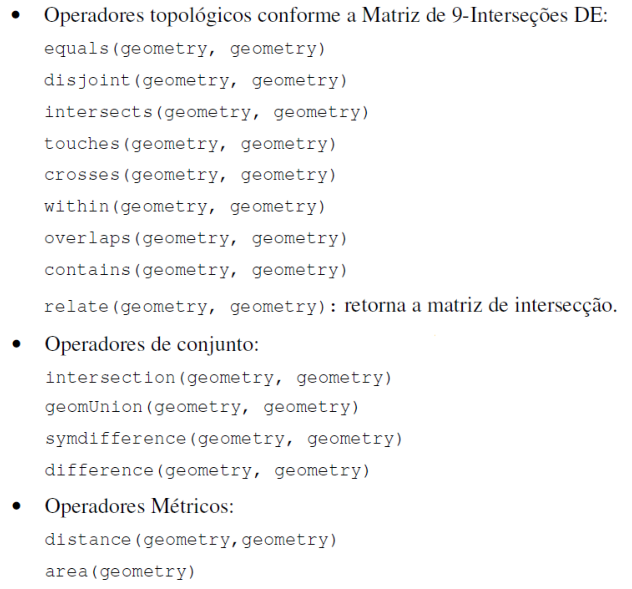
\includegraphics[width=0.70\textwidth]{./img/cap_II/16-OperadoresPostGIS}
\caption{Operadores espaciais disponíveis no PostGIS, adaptado de \cite{queirozferreira}.}
\label{fig:OperadoresPostGIS}
\end{figure}

\newpage

Em \citeonline{spatialjoins}, as consultas espaciais são classificadas nos seguintes itens:

\begin{itemize}
\item Seleção espacial: determina todos os objetos de um conjunto de objetos espaciais cujas geometrias satisfazem um predicado de seleção espacial;
\item Junção espacial: determina todos os pares de dois conjuntos de objetos espaciais cujas geometrias satisfazem um predicado de seleção espacial.
\end{itemize}

São identificados casos particulares importantes na seleção espacial \cite{spatialjoins}:

\begin{itemize}
\item Seleção por ponto: determina todos os objetos de um conjunto de objetos espaciais cujas geometrias contêm um ponto dado;
\item Seleção por região: determina todos os objetos de um conjunto de objetos espaciais cujas geometrias estão contidas em uma região dada;
\item Seleção por janela: determina todos os objetos de um conjunto de objetos espaciais cujas geometrias estão contidas em um retângulo com os lados paralelos aos eixos dados.
\end{itemize}

A Figura \ref{fig:SelecaoEspacial} apresenta o resultado de uma seleção espacial. Na Figura é selecionado as regiões da França adjacentes à região de \textit{Midi-Pirenées} (a região de \textit{Midi-Pirenées} aparece em cinza escuro e as regiões adjacente em cinza claro).

\begin{figure}[h]
\centering
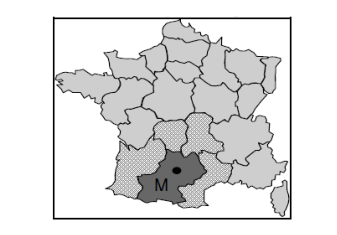
\includegraphics[width=0.50\textwidth]{./img/cap_II/17-SelecaoEspacial}
\caption{Operação de seleção espacial \cite{queirozferreira}.}
\label{fig:SelecaoEspacial}
\end{figure}

A Figura \ref{fig:JuncaoEspacial} apresenta o resultado de um junção espacial. Na consulta é utilizado o operador  espacial \textit{SDO\_TOUCH} que retorna verdadeiro caso as geometrias de d2 toquem a geometria de Grajaú. Esse é um exemplo de junção espacial entre duas relações (no nosso caso a mesma relação foi empregada duas vezes), utilizando o índice espacial \cite{queirozferreira}.

\newpage

\begin{figure}[h]
\centering
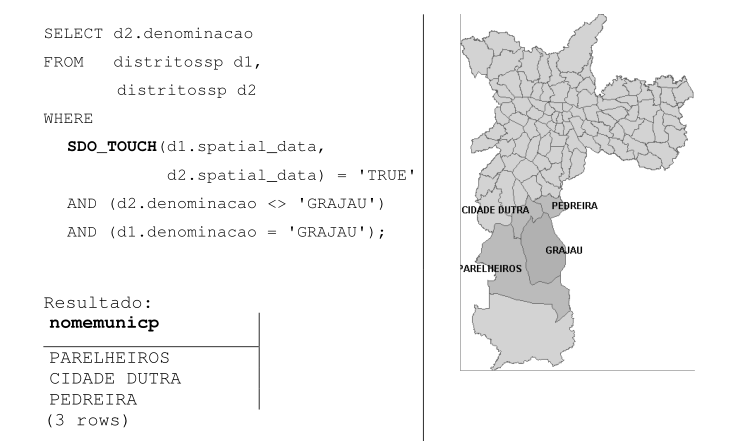
\includegraphics[width=0.75\textwidth]{./img/cap_II/19-JuncaoEspacial}
\caption{Operação de junção espacial \cite{queirozferreira}.}
\label{fig:JuncaoEspacial}
\end{figure}
\chapter{Sistema de Informação Geográfico}
\label{cap:sig}

\section{Introdução}

O termo Sistemas de Informação Geográfico (SIG) é aplicado para sistemas que realizam o tratamento computacional de dados geográficos. A principal diferença de um SIG para um sistema de informação convencional é sua capacidade de armazenar tanto os atributos descritivos como as geometrias dos diferentes tipos de dados geográficos \cite{camara}.

O SIG é usado frequentemente em projetos e pesquisas ambientais e urbanas, análise de mercado, monitoramento de recursos naturais, e também por outros profissionais cujo trabalho se baseia em mapas, possibilitando uma visão geral de seu ambiente de trabalho, em que todas as informações de uma base determinada estão ao seu alcance. Este trabalho é possível por meio do georreferenciamento da geometria e os atributos dos dados, ou seja, a localização na superfície terrestre e representados em uma projeção cartográfica \cite{websisbra}.

Em \citeonline{queirozferreira}, é apresentada as principais características de um SIG:

\begin{itemize}
\item Inserir e integrar, em uma única base de dados, informações espaciais provenientes de meio físico-biótico, de dados censitários, de cadastros urbano e rural, e outras fontes de dados como imagens de satélite, e  Sistema de Posicionamento Global (GPS);
\item Oferecer mecanismos para combinar as várias informações, através de algoritmos de manipulação e análise, bem como para consultar, recuperar e visualizar o conteúdo da base de dados geográficos.
\end{itemize}

Nas seções deste capítulo, são abordados os principais conceitos relacionados a função de um SIG, arquitetura de um SIG, integração de arquiteturas SIG, SIG Web, arquitetura de um SIG Web, padrões de desenvolvimento de um SIG, Infraestrutura Nacional de Dados Espaciais (INDE) e \textit{Open Geospatial Consortium} (OGC).

\section{Função de um SIG}

O principal aspecto de um SIG reside na forma de como aplicar e agrupar um conjunto de dados e informações para a solução de um determinado problema. Devido a sua ampla gama de aplicações, que incluem temas como agricultura, cadastro urbanos ou rurais, por exemplo, há pelo menos três grandes maneiras de utilizar um SIG \cite{websisbra}:

\begin{itemize}
\item Produção de mapas;
\item Suporte para análise espacial de fenômenos;
\item Banco de dados geográficos, com funções de armazenamento e recuperação de informação espacial.
\end{itemize}

\newpage

É possível aplicar uma diversidade de soluções em um SIG. As características mais comuns são \cite{zeiler}:

\begin{itemize}
\item Integração do SIG com outras aplicações para execução de análise geográfica e científica. Os dados do SIG precisam estar estruturados e armazenados de modo a permitir o acesso aos dados distribuídos;
\item Arquitetura de informação aberta é essencial, pois facilita a integração de dados geográficos com outros dados;
\item Acesso interativo proporciona os mais sofisticados modelos de dados no apoio às questões e análises;
\item Estrutura de dados adequada ao tipo de análise executada. Tal como uma imagem (representação matricial) ou como conjunto dados em formato vetorial.
\end{itemize}

\section{Arquitetura de um SIG}

A arquitetura de um SIG é composto pelos seguintes componentes: interface, entrada e integração de dados, consulta e análise espacial, visualização e plotagem, e por fim, gerência de dados espaciais.

Cada sistema pode implementar estes componentes de forma distinta, mas todos os subsistemas citados devem estar presentes em um SIG \cite{camara}. A Figura \ref{fig:ArquiteturaSIG} apresenta os componentes de um SIG.

No nível mais próximo ao usuário, a interface homem-máquina define como o sistema é operado e controlado. Esta interface pode ser tanto baseada em ambientes \textit{desktops} ou ambientes que possuam navegação com a Internet. No nível intermediário, um SIG deve ter mecanismos de processamento de dados espaciais. A entrada de dados inclui os mecanismos de conversão de dados. Os algoritmos de consulta e análise espacial incluem as operações topológicas, álgebra de mapas, estatística espacial, modelagem numérica de terreno e processamento de imagens. Os mecanismos de visualização e plotagem, devem oferecer suporte adequado para a apreensão cognitiva dos aspectos relevantes dos dados pesquisado. No nível mais interno do sistema, um sistema de gerência de bancos de dados geográfico oferece armazenamento e recuperação dos dados espaciais e seus atributos \cite{camara}.

\begin{figure}[h]
\centering
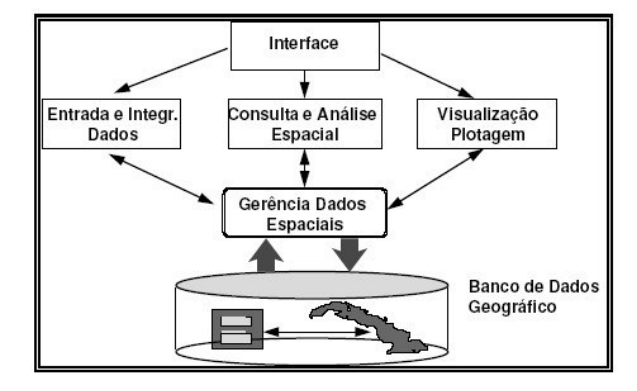
\includegraphics[width=0.65\textwidth]{./img/cap_III/1-ArquiteturaSIG}
\caption{Componentes de um SIG \cite{camara}.}
\label{fig:ArquiteturaSIG}
\end{figure}

Do ponto de vista da aplicação, o uso de um SIG implica em escolher as representações computacionais mais adequadas para capturar a semântica de seu domínio de aplicação. Do ponto de vista da tecnologia, desenvolver um SIG significa oferecer o conjunto mais amplo possível de estruturas de dados e algoritmos capazes de representar a grande diversidade de concepções do espaço \cite{camara}.

\subsection{Modelos de Arquiteturas SIG}

Existem duas principais integrações na arquitetura de um SIG: arquitetura dual e arquitetura integrada. Ambas são definidas a partir da integração entre SIGs e SGBDs \cite{queirozferreira}.

A arquitetura dual representada pela Figura \ref{fig:ArquiteturaDual}, armazena os dados espaciais separadamente dos dados convencionais, ou seja, os dados convencionais são armazenados em um SGBD relacional e os dados espaciais são armazenados em arquivos com formato proprietário. Essa arquitetura ocasiona vários problemas \cite{queirozferreira}:

\begin{itemize}
\item Dificuldade no controle e manipulação dos componentes espaciais;
\item Dificuldade em manter a integridade entre o componente espacial e o componente alfanumérico;
\item Separação entre o processamento da parte convencional, realizado pelo SGBD, e o processamento da parte espacial, realizado pelo aplicativo utilizando os arquivos proprietários;
\item Dificuldade de interoperabilidade, já que cada sistema trabalha com arquivos com formato proprietário.
\end{itemize}

\begin{figure}[h]
\centering
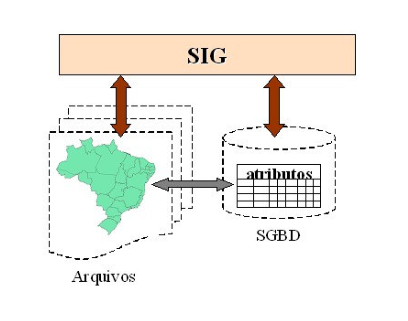
\includegraphics[width=0.50\textwidth]{./img/cap_III/2-ArquiteturaDual}
\caption{Arquitetura dual \cite{queirozferreira}.}
\label{fig:ArquiteturaDual}
\end{figure}

A Figura \ref{fig:ArquiteturaIntegrada} apresenta a arquitetura integrada, que consiste em armazenar todos os dados em um SGBD, ou seja, tanto o componente espacial quanto o alfanumérico. Sua principal vantagem é a utilização dos recursos de um SGBD para controle e manipulação de objetos espaciais, como gerência de transações, controle de integridade, concorrência e linguagens próprias de consulta. Sendo assim, a manutenção de integridade entre o componente espacial e o alfanumérico é feita pelo SGBD \cite{queirozferreira}.

\newpage

\begin{figure}[h]
\centering
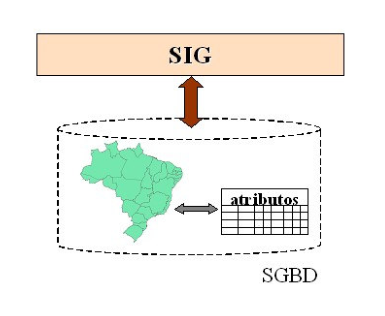
\includegraphics[width=0.50\textwidth]{./img/cap_III/3-ArquiteturaIntegrada}
\caption{Arquitetura integrada \cite{queirozferreira}.}
\label{fig:ArquiteturaIntegrada}
\end{figure}

A arquitetura integrada pode ainda ser subdividida em três outras: baseada em campos longos, em extensões espaciais e combinada \cite{queirozferreira, bancogeo}.

A arquitetura integrada baseada em campos longos utiliza BLOBs (cadeia de bits sem nenhuma semântica adicional) para armazenar os dados espaciais. As desvantagens do uso do BLOB é que ele não possui semântica e não possui métodos de acesso \cite{queirozferreira}.

A arquitetura integrada com extensões espaciais consiste em utilizar extensões espaciais desenvolvidas sobre um Sistema Gerenciador de Banco de Dados Objetos-Relacionais (SGBD-OR). Essa arquitetura permite definir tipos de dados espaciais com operadores específicos e métodos de acesso específicos para dados espaciais, o que a torna muito vantajosa em relação à outra arquitetura. Um exemplo dessa arquitetura é o PostGIS que foi abordado no capítulo anterior deste trabalho \cite{queirozferreira}.

A arquitetura integrada combinada é formada pela combinação das duas anteriores, é utilizada por SIGs que manipulam dados espaciais com geometrias matriciais e vetoriais, as geometrias vetoriais são armazenadas pelos recursos das extensões espaciais e as geometrias matriciais são armazenadas em BLOBs \cite{queirozferreira}.

\section{SIG Web}

A principal característica de um SIG é a capacidade de representar atributos espaciais, além dos atributos convencionais (alfanuméricos). Essa característica adicional permite ilustrar relações, conexões e padrões que não são facilmente visíveis em qualquer conjunto de dados, essa característica torna mais fácil a tomada de decisões nas organizações.

É considerado um SIG Web, qualquer SIG que utiliza tecnologias da Web para interação de dados geográficos, permitindo a visualização dos dados através do uso do \textit{browser}. A utilização do SIG Web permite que o usuário interaja constantemente com o sistema, considerando a facilidade de acesso através de um \textit{browser}, podendo assim, a possibilidade de ser acessado de qualquer dispositivo móvel por exemplo \cite{webgis}.

\newpage

\section{Arquitetura de um SIG Web}

A arquitetura de um SIG Web mais usada é baseada em três camadas: camada de interface, camada de servidor de aplicação e a camada de banco de dados \cite{webgisfuture}. A Figura \ref{fig:ArquiteturaSIGWeb} apresenta a arquitetura de um SIG Web.

\begin{figure}[h]
\centering
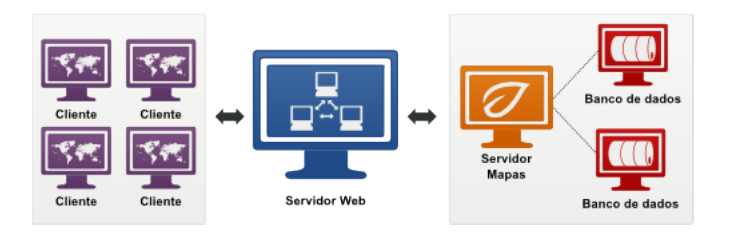
\includegraphics[width=0.65\textwidth]{./img/cap_III/4-ArquiteturaSIGWeb}
\caption{Arquitetura de um SIG Web \cite{websisbra}.}
\label{fig:ArquiteturaSIGWeb}
\end{figure}

\begin{itemize}
\item A Camada de Interface, também conhecida como Camada do Cliente, é a camada responsável por apresentar os dados espaciais no \textit{browser} do usuário. Através da apresentação desses dados, os usuários interagem com os serviços oferecidos pelo SIG Web;
\item A Camada de Servidor de Aplicação é responsável por realizar a comunicação  com as fontes de dados, permitindo o usuário final de analisar e manipular esses dados;
\item A Camada de Banco de Dados faz uso de um banco de dados geográficos para relacionar atributos convencionais e atributos geográficos. Esta camada possui um conjunto de serviços de provedores de dados remotos que são utilizados pelo SIG Web, fazendo que cada banco de dados ofereça um conjunto de interfaces para as aplicações clientes fazerem uso dos dados remotamente.
\end{itemize}

Um SIG Web pode ser desenvolvido a partir de um modelo de arquitetura cliente-servidor, do tipo \textit{thin client} ou \textit{thick client}. O modelo  \textit{thin client}, representado na Figura \ref{fig:ArquiteturaThinClient}, o cliente tem acesso ao servidor somente através da interface de interação para obter as informações. Todo o processamento da aplicação é feito no lado do servidor, que, geralmente, é um computador com maiores recursos computacionais do que o do cliente, de forma a centralizar os recursos \cite{websisbra}.

\begin{figure}[h]
\centering
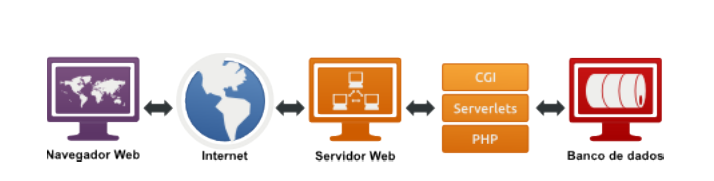
\includegraphics[width=0.70\textwidth]{./img/cap_III/5-ArquiteturaThinClient}
\caption{Modelo de arquitetura \textit{thin client} \cite{websisbra}.}
\label{fig:ArquiteturaThinClient}
\end{figure}

Algumas vantagens no uso desse tipo de arquitetura são:

\begin{itemize}
\item Software centralizado;
\item Facilidade de manutenção;
\item Facilidade de atualização;
\item Controle de acesso simples.
\end{itemize}

Algumas das desvantagens são:

\begin{itemize}
\item Pode ter um tempo de resposta longo;
\item Dados vetoriais não são renderizados no lado do cliente sem que haja a necessidade de ter que instalar algum \textit{plugin} adicional;
\item Grande volume de dados devido a taxa constante de transmissão;
\item Processamento pelo servidor a toda tarefa requisitada, até ações mais simples como: \textit{zoom}, mover e selecionar.
\end{itemize}

A Figura \ref{fig:ArquiteturaThickClient} representa o modelo \textit{thick client}, nesse modelo parte do processamento da aplicação que é executada pelo cliente. Diferente de um \textit{thin client}, esse modelo processa o maior número de informações na camada do cliente, e passa ao servidor somente dados necessários para comunicação e o armazenamento de arquivos. Os navegadores de Internet tem papel fundamental nesse tipo de arquitetura. São clientes leves, capazes de exibir o conteúdo e oferecem suporte a tecnologias que possibilitam a interação com o usuário, como Javascript ou através da adição de \textit{plugins} ou \textit{applets} \cite{websisbra}.

Algumas vantagens no uso desse tipo de arquitetura são:

\begin{itemize}
\item Redução na carga no servidor, usando processamento no cliente;
\item Redução no tráfego da rede, pois os dados podem ser processados localmente;
\item Fácil controle de tarefas simples por parte do cliente (\textit{zoom}, mover, selecionar);
\item Fácil manipulação de mapas vetoriais.
\end{itemize}

Algumas das desvantagens são:

\begin{itemize}
\item Instalação de plugins ou applets;
\item Computador do cliente pode ter um poder de processamento baixo;
\item Carrega, inicialmente, uma quantidade maior de dados.
\end{itemize}

\begin{figure}[h]
\centering
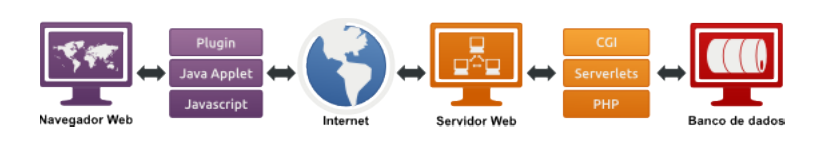
\includegraphics[width=0.75\textwidth]{./img/cap_III/6-ArquiteturaThickClient}
\caption{Modelo de arquitetura \textit{thick client} \cite{websisbra}.}
\label{fig:ArquiteturaThickClient}
\end{figure}

\section{Padrões Para o Desenvolvimento de um SIG}

O emprego de dados geoespaciais, ou seja, dados referenciados à superfície terrestre, é cada vez mais intenso, tanto por usuários públicos quanto privados. O atendimento a essa demanda exige que a produção e a disseminação desses dados sejam realizados de forma ágil. O atual estágio das geotecnologias, como o sensoriamento remoto, o posicionamento por satélites, os sistemas de produção cartográfica, os sistemas de informações geográficos e o acesso à Web (\textit{webmapping}), tem acelerado ainda mais este processo \cite{concar}.

Nesta seção será descrita os principais padrões para desenvolvimento de um SIG.

\subsection{Infraestrutura Nacional de Dados Espaciais}

A Infraestrutura Nacional de Dados Espaciais (INDE) é o conjunto integrado de tecnologias, políticas, mecanismos e procedimentos de coordenação e monitoramento, padrões e acordos, necessário para facilitar e ordenar a geração, o armazenamento, o acesso, o compartilhamento, a disseminação e o uso dos dados geoespaciais de origem federal, estadual, distrital e municipal \cite{inde}.

Dentre as especificações da INDE deve estar presente uma que defina propriadamente a estrutura empregada na aquisição e armazenamento de informações geoespaciais, que permita a disseminação e a disponibilização, otimizando assim o seu compartilhamento, e maximizando a utilidade dos recursos da Tecnologia da Informação, nos diferentes níveis de governo, no setor privado, no terceiro setor, na comunidade acadêmica e na Sociedade como um todo. Para isso, a INDE modelou a estrutura de dados geoespaciais vetoriais utilizando a técnica de modelagem conceitual OMT-G \cite{concar}.

O domínio desse trabalho, SIG Web, não foi especificado pela INDE, logo o modelo conceitual do SIG Web desenvolvido não seguiu nenhuma especificação, foi feito livremente.

\subsection{Open Geospatial Consortium}

\textit{Open Geospatial Consortium} (OGC) é uma organização voluntária internacional de padrões de consenso. Na OGC, mais de 400 organizações comerciais, governamentais, não lucrativas e instituições de pesquisa do mundo todo colaboram num processo de consenso aberto encorajando o desenvolvimento e a implementação de padrões para conteúdo e serviços geomáticos, SIG, processamento e troca de dados. Os padrões estabelecidos pela OGC suportam soluções interoperáveis baseadas na internet e que também são desenvolvidos para trabalhar com informações espaciais complexas e serviços utilizados por diferentes tipos de aplicações \cite{ogc}.

Os padrões atualmente aprovados pela OGC estão agrupados em conjuntos temáticos de serviços de catálogo, serviços de processamento, codificação, serviços de dados, serviços de retrato (imagem) e outros padrões comuns. Em seguida, são descritos os mais importantes \cite{harley, ogc}:

\begin{itemize}
\item \textit{Geographic Markup Language} (GML): Um padrão de codificação baseado em \textit{eXtensible Markup Language} (XML) para informações geográficas desenvolvidas pelo consórcio OGC. A GML foi especificada para o transporte e armazenamento de informação geográfica, incluindo propriedades espaciais e não espaciais das feições geográficas. O objetivo da GML é oferecer um conjunto de regras com as quais um usuário pode definir seu esquema para descrever seus dados. Sua versão 3.0 inclui esquemas que contêm os modelos de geometria, feições e superfícies;
\item \textit{Keyhole Markup Language} (KML): uma notação XML para exibir dados geográficos em um navegador da Terra, como \textit{Google Earth}, \textit{Google Maps}. O KML utiliza uma estrutura de marcadores com elementos e atributos aninhados e se baseia no padrão XML. KML foi desenvolvido para uso com o \textit{Google Earth}, sendo originalmente chamado \textit{Keyhole Earth Viewer}. Foi criado por \textit{Keyhole Inc.} sendo um padrão internacional da OGC, o arquivo KML especifica um conjunto de características (marca local, imagens, polígonos, modelos 3D, descrições textuais, entre outros) para exibição no \textit{Google Earth}, \textit{Maps} e \textit{Mobile}. O KML compartilha algumas das mesmas gramáticas estruturais como GML.

\newpage

\item \textit{Web Map Service} (WMS): é um padrão que fornece uma interface \textit{Hypertext Transfer Protocol} (HTTP) simples para solicitar imagens de mapas georreferenciadas de um ou mais bancos de dados geoespaciais distribuídos. A solicitação WMS define as camadas geográfica(s) e área de interesse a ser processado. A resposta ao pedido é uma ou mais imagens georreferenciadas do mapa (retornado como JPEG, PNG) que podem ser exibidos em um navegador. A interface também suporta a capacidade para especificar se as imagens retornadas devem ser transparentes ou não para que as camadas de vários servidores possam ser combinadas.
\item \textit{Web Feature Services} (WFS): é um serviço padrão, que fornece uma interface de comunicação que permite interagir com mapas atendidos pelo padrão WMS, por exemplo, editar a imagem oferecida pelo serviço WMS ou analisar a imagem usando critérios geográficos. Para realizar essas operações, utiliza-se GML linguagem derivada do XML, que é o padrão pelo qual são transmitidas as ordens WFS, no entanto, qualquer outro formato vetorial pode ser utilizado. WFS não transacional permite a consulta e recuperação de recursos geográficos. Pelo contrário, \textit{Web Feature Service Transacional} (WFS-T) permite também criar, apagar e atualizar esses recursos de mapas geográficos.
\item \textit{Web Coverage Service} (WCS): define uma interface padrão e operações que permitem o acesso interoperável para dados geoespaciais do tipo “matriz”. O termo “matriz” normalmente refere-se a conteúdos como imagens de satélite, fotos aéreas digitais e dados de elevação digital. Este padrão também possui a definição de operação de transação, onde opcionalmente pode ser implementado por servidores WCS. Esta operação de transação permite ao usuário adicional, modificar e eliminar dados matriciais num servidor WCS. As referências de transação ou operação de solicitação incluem a criação de novo dado matricial ou modificações de um existente, abrangendo todos os metadados necessários para um dado matricial.
\end{itemize}
\chapter{SIG Web Luziânia}
\label{cap:sigluziania}

\section{Introdução}

O SIG Web Luziânia é um SIG Web com a finalidade de gerenciar e visualizar  dados de serviços básicos da cidade de Luziânia, os quais são: educação, lazer, saúde e segurança. Além disso, organizar os dados em um banco de dados geográfico para que seja inserida a geometria da localização exata de cada serviço básico.

Em um primeiro momento, foi realizado a coleta de dados de todos os serviços. Essa coleta foi realizada através de dados disponibilizados pela prefeitura do município, dados públicos encontrados na Internet e através de conhecimento empírico da localização dos serviços coletados.

Os dados relacionados a educação são de escolas, faculdades e escolas técnicas, todas distribuídas no âmbito municipal, estadual, federal e privado. Através de gráficos é visualizado informações disponibilizadas pelo Ministério da Educação (MEC), com as notas das instituições de ensino nas avaliações do Exame Nacional do Ensino Médio (ENEM) e do Índice de Desenvolvimento da Educação Básica (IDEB).

Os dados sobre saúde são de hospitais e postos de saúde, contendo as especialidades médicas presentes em cada um dos hospitais ou postos de saúde. Os dados sobre lazer são de localidades que envolvem entretenimento, entre elas: praças, quadras poliesportivas, teatro, cinema, restaurante, e bares. Os dados sobre segurança são de delegacias, presídios, órgãos de justiça e batalhões policiais.

O SIG Web Luziânia foi desenvolvido usando apenas tecnologias livres para uso. O sistema foi desenvolvido na linguagem de programação C\#, junto com o \textit{framework} de desenvolvimento Web \textit{ASP.NET MVC}. No sistema é possível visualizar e interagir com os dados de uma maneira rápida e segura, além de ser possível a criação de novos dados. O sistema é totalmente acessível em dispositivos móveis, sendo possível a população do município acessar de qualquer lugar necessitando apenas de acesso à Internet.

\section{Aplicação dos Quatro Universos}

Nesta seção é descrito como foi aplicado a metodologia dos quatro universos no desenvolvimento do SIG Web Luziânia.

\subsection{Universo Ontológico}
\label{universo-ontologico}

Para o desenvolvimento de um SIG Web é necessário escolher as entidades a serem representadas, assim com a sua descrição. Uma geo-ontologia é um conjunto de conceitos e das relações semânticas e espaciais entre esses termos \cite{gisasp}. A primeira etapa de desenvolvimento do SIG Web Luziânia foi a construção de sua geo-ontologia. Os conceitos relacionados com o SIG Web Luziânia são de dois tipos:

\begin{itemize}
\item O primeiro tipo, envolve os conceitos associados às entidades não geográficas;
\item O segundo tipo, os conceitos associados às entidades geográficas criadas pelos seres humanos para representar entidades sociais e institucionais que descrevem entidades individuais criadas por ação e por leis. Essas entidades possuem uma identidade única e uma fronteira que as distinguem do mundo ao seu redor.
\end{itemize}
	
As entidades identificadas nesse cenário para o desenvolvimento do SIG Web Luziânia foram: 

\begin{itemize}
\item Usuário: pessoa responsável pelo controle dos dados do sistema;
\item Perfil: define o tipo de acesso do usuário ao sistema;
\item Cidade: localidade onde os dados serão georreferenciados;
\item Educação: localidades relacionadas as instituições de ensino;
\item Avaliação: avaliações escolares vinculadas as instituições de ensino;
\item Segurança: localidades relacionadas a segurança;
\item Tipo Segurança: tipo de localidade de segurança (delegacias, presídios, órgãos de justiça e batalhões policiais);
\item Lazer: localidades relacionadas ao entretenimento;
\item Tipo Lazer: tipos de localidades de entretenimento (praças, quadras poliesportivas, teatro, cinema, restaurante, e bares);
\item Saúde: localidades relacionadas a saúde;
\item Tipo Saúde: tipos de localidades de saúde (hospitais e postos de saúde);
\item Especialidade: especialidades médicas vinculadas as localidade de saúde.
\end{itemize}

\subsection{Universo Formal}

O paradigma dos quatro universos trata apenas do problema da representação computacional do espaço, por esse motivo será realizada apenas a passagem do universo ontológico para o universo formal das entidades geográficas do SIG Web Luziânia, ou seja, dos conceitos com características geográficas. Apenas os conceitos de educação, lazer, saúde e segurança possuem características geográficas no SIG Web Luziânia.

A passagem do universo ontológico para o universo formal caracteriza em representar um conceito genérico no qual é definido os atributos que caracterizam esse conceito e como pode-se medir o seu território. O processo de medida consiste em associar números ou símbolos a diferentes ocorrências de um mesmo atributo, a fim de que a relação dos números ou símbolos reflitam essas variações. Para medir os conceitos de educação, lazer, saúde e segurança do SIG Web Luziânia, foi utilizado a escala de medida nominal que classifica objetos em classes distintas, como rótulos que podem ser qualquer símbolos, como por exemplo, a cobertura do solo, que tem rótulos como floresta, área urbana e área agrícola.

O conceito das entidades educação, lazer, saúde e segurança foi medido a partir da presença de localidades caracterizadas e partir de cada entidade. Esse conceito é modelado no espaço absoluto porque a localização exata é fundamental para esses conceitos. Existem dois modelos formais para entidades geográficas no espaço absoluto: geo-campos e geo-objetos.

As entidades educação, lazer, saúde e segurança foram modelados como geo-objetos porque são entidades distintas e identificáveis, cada entidade é definida por uma fronteira.

\subsection{Universo Estrutural}

Para passar do universo formal para o universo estrutural é necessário relacionar cada tipo de entidade do modelo formal a estruturas de dados do universo estrutural. Para cada tipo de entidade do modelo formal, há diferentes possibilidades de uso de estruturas de dados.

Todas as entidades geográficas do SIG Web Luziânia (educação, lazer, saúde e segurança) utilizaram a estrutura vetorial ponto para representar as coordenadas das suas fronteiras, porque o ponto representa ocorrências ou localizações no espaço. No caso específico das entidades geográficas presentes no sistema, todas representam localizações.

\subsection{Universo de Implementação}

O SIG Web Luziâna foi desenvolvido na arquitetura cliente-servidor, ou seja, clientes requisitam serviços aos servidores que provem serviços, estando interligados entre si utilizando uma rede de computadores, nesse caso específico, a Internet. Ele é dividido em duas partes: a parte georreferenciada, principal funcionalidade do sistema, e a parte administrativa responsável pelo controle dos dados que alimenta a base de dados utilizada na primeira parte.

O SIG Web Luziânia possui um banco de dados geográfico que foi implementado no SGBD PostgreSQL utilizando a extensão espacial PostGIS. A alimentação dos dados é realizada na parte administrativa do sistema, através do preenchimento manual dos formulários existentes no sistema.

A visualização dos dados georreferenciados no mapa ocorre na integração da comunicação \textit{RESTful} e a biblioteca Javascript \textit{Leaflet}.

O sistema foi desenvolvido utilizando o \textit{framework} de desenvolvimento Web \textit{ASP.NET MVC}, juntamente com a linguagem de programação C\# e Javascript para realizar validações do sistema.

\section{Modelo de Dados}

A estrutura do banco de dados geográfico do SIG Web Luziânia foi definida a partir de dois modelos de dados: o conceitual e o lógico. O modelo conceitual fornece uma abstração mais alta dos dados, no nível de usuário. O modelo lógico, descreve como os dados serão armazenados no SGBD.
O modelo de dados OMT-G é o padrão definido pela INDE para modelagem de dados conceituais \cite{inde}. O modelo OMT-G foi utilizado para a criação do modelo conceitual, o qual foi abordado na seção \ref{modelo-omtg} deste trabalho. A Figura \ref{fig:DiagramaOMTG} apresenta o modelo OMT-G do SIG Web Luziânia e suas respectivas entidades identificadas. 

Para o entendimento dos relacionamentos entre as entidades, foi utilizado o conceito de entidades apresentados na seção \ref{universo-ontologico}. Na Tabela \ref{tabela-omtg} é visualizada a explicação para cada relacionamento do modelo OMT-G.

Para a criação do esquema do banco de dados do SIG Web Luziânia em um SGBD é necessário transformar o modelo conceitual em um modelo lógico. Essa transformação consiste no mapeamento do modelo OMT-G para o modelo relacional (MR) que representa os dados em um banco de dados como uma coleção de relações (tabelas). A Figura \ref{fig:ModeloER} apresenta o modelo conceitual do SIG Web Luziânia que foi criado a partir desse mapeamento. As chaves douradas e vermelhas, representam respectivamente as chaves primárias e estrangeiras.

\newpage

\begin{figure}[h]
\centering
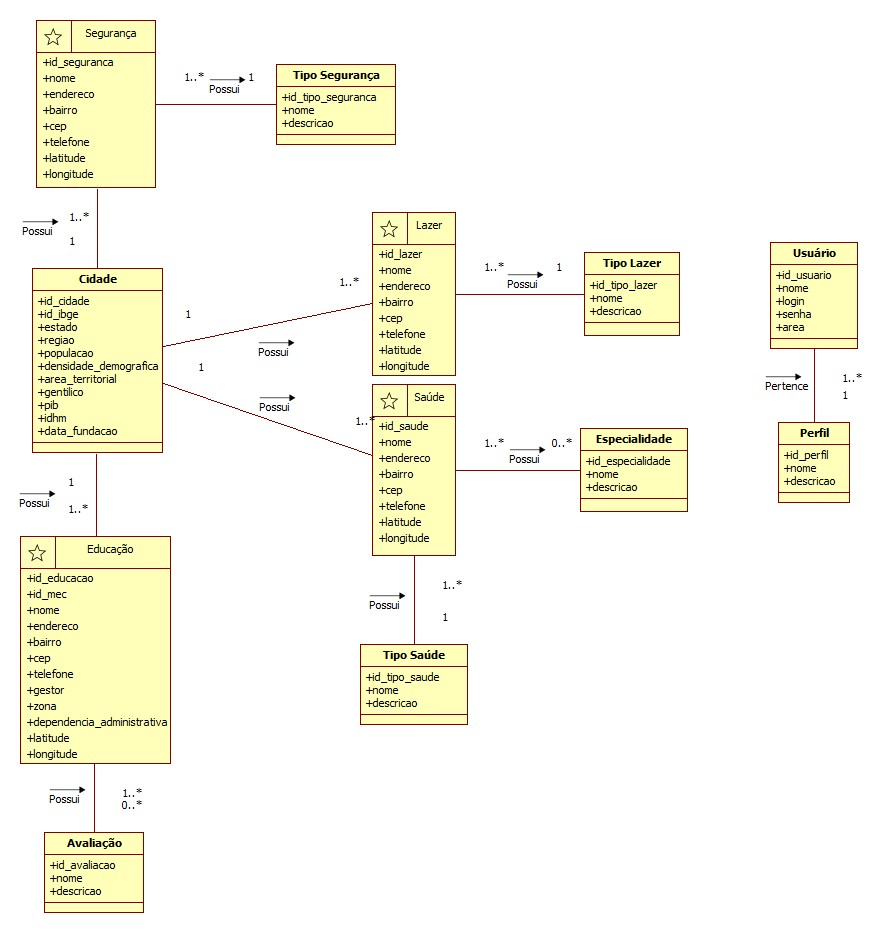
\includegraphics[width=0.69\textwidth]{./img/cap_IV/1-DiagramaOMTG}
\caption{Modelo OMT-G do SIG Web Luziânia.}
\label{fig:DiagramaOMTG}
\end{figure}

\begin{table}[htb]
\IBGEtab{
\caption{Explicação do modelo OMT-G do SIG Web Luziânia.}
\label{tabela-omtg}
}{
\begin{tabular}{ll}
\toprule
Relacionamento & Descrição\\
\midrule \midrule
Usuário e Perfil & Usuário pertence a um perfil, e um perfil pertence a vários usuários\\
\midrule
Cidade e Educação & Cidade possui instituições de ensino, instituições de ensino pertence a uma cidade\\
\midrule
Educação e Avaliação & Instituições de ensino possui uma avaliação ou várias, avaliação pertence\\
& a uma ou várias instituições de ensino\\
\midrule
Cidade e Segurança & Cidade possui localidades de segurança, localidades de segurança\\
& pertence a uma cidade\\
\midrule
Segurança e Tipo Segurança & Localidades de segurança possui um tipo específico, um tipo possui\\
& uma ou várias localidades de segurança\\
\midrule
Cidade e Lazer & Cidade possui dados de entretenimento, dados de entretenimento pertence a uma cidade\\
\midrule
Lazer e Tipo Lazer & Dados de entretenimento possui um tipo específico, um tipo possui\\
& um ou vários dados de entretenimento\\
\midrule
Cidade e Saúde & Cidade possui localidades de saúde, localidades de saúde pertence a uma cidade\\
\midrule
Saúde e Tipo Saúde & Localidades de saúde possui um tipo específico, um tipo possui\\
& uma ou várias localidades de saúde\\
\midrule
Saúde e Especialidade & Localidades de saúde possui uma especialidade ou várias, especialidade possui\\
& uma ou várias localidades de saúde\\
\bottomrule
\end{tabular}}{}
\end{table}

\newpage

\begin{figure}[h!]
\centering
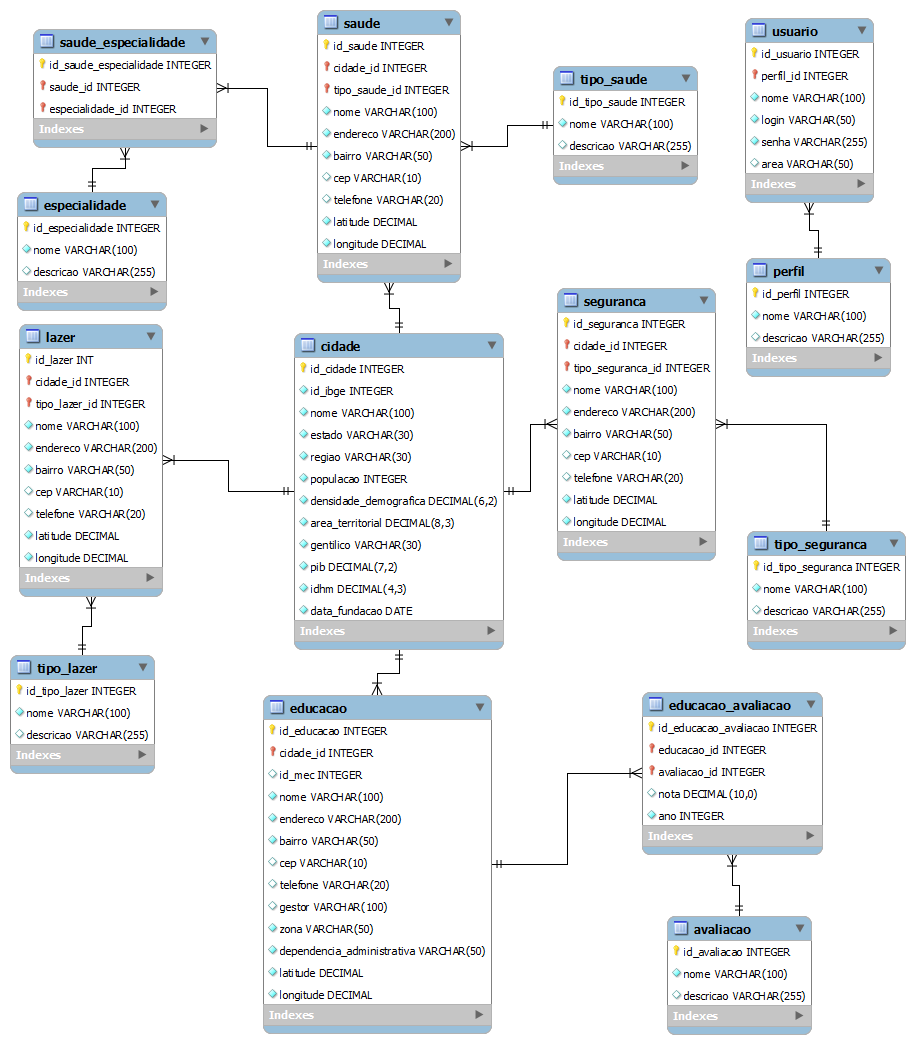
\includegraphics[width=0.75\textwidth]{./img/cap_IV/2-ModeloER}
\caption{Modelo relacional do SIG Web Luziânia.}
\label{fig:ModeloER}
\end{figure}

\section{Implementação}

Nesta seção é abordada questões relacionadas a implementação do SIG Web Luziânia, a arquitetura do sistema e as tecnologias utilizadas.

\subsection{Arquitetura do SIG Web Luziânia}

A arquitetura abstrata do SIG Web Luziânia é representada na Figura \ref{fig:arquiSig}, utilizando o tipo de arquitetura \textit{thick client} (definida no capítulo \ref{cap:sig}) e sendo composta por três grandes módulos: Camada de Interface, Camada de Aplicação e Camada de Persistência.

\begin{itemize}
\item A Camada de Interface é responsável pela interação do sistema com o usuário através de formulários e da visualização dos dados;
\item A Camada de Aplicação é responsável pelo mecanismo de gerar os dados do mapa;
\item A Camada de Persistência é responsável pelo tratamento e armazenamento dos dados em um SGBD.
\end{itemize}

\newpage

\begin{figure}[h]
\centering
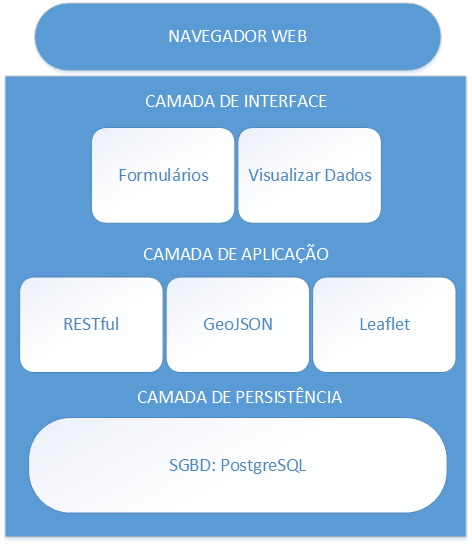
\includegraphics[width=0.55\textwidth]{./img/cap_IV/3-ArquiteturasSigLuziania}
\caption{Arquitetura abstrata do SIG Web Luziânia.}
\label{fig:arquiSig}
\end{figure}

O usuário interage com a Camada de Interface a partir de um navegador web. Ao acessar a página inicial do sistema, o usuário irá visualizar os dados georreferenciados plotados no mapa, além de visualizar esses dados com mais detalhes nos formulários apresentados na página inicial. A área administrativa do sistema possui formulários para inserção, visualização, atualização e deleção dos dados.

A camada de aplicação é responsável por gerar os dados que serão plotados no mapa. Essa camada é composta pelo sistema \textit{RESTful} \cite{restful} e para comunicação desse sistema é usado o \textit{framework ASP.NET Web API} \cite{webapi}, responsável em prover serviços Web utilizando a abordagem \textit{RESTful}. O formato da saída dos dados realizada na chamada \textit{RESTful} é o \textit{Javascript Object Notation} (JSON) \cite{json}.

\textit{GeoJSON} é responsável por codificar estruturas de dados geográficos fazendo uso do formato JSON. O \textit{GeoJSON} suporta os principais dados espaciais, sendo eles: ponto, linha, polígono multipontos, multilinhas, multipolígonos, coleções geométricas, características e listas de características \cite{geojson}. Por ser baseado no formato JSON os dados são armazenados de maneira mais organizada e mais compacta do que o formato XML, por exemplo.

O \textit{Leaflet} é uma biblioteca \textit{open source} em Javascript para criação de mapas interativos aproveitando as novas tecnologias em navegadores modernos \cite{leaflet}. O \textit{Leaflet} faz uso do \textit{GeoJSON} para visualização dos dados gerados.

Por fim, a Camada de Persistência é responsável pelo armazenamento dos dados do sistema. Os dados são armazenados no SGBD PostgreSQL, com a extensão espacial PostGIS para o armazenamento dos dados geográficos.

\newpage

\subsection{Tecnologias Utilizadas}

\subsubsection{C\#}

O C\# (pronuncia-se "C sharp") é uma linguagem de programação interpretada orientada a objetos, fortemente tipada e altamente escalável. O C\# é uma linguagem de programação criada para o desenvolvimento de aplicações que executam o \textit{framework .NET} \cite{csharp}.

A linguagem C\# é uma linguagem multiplataforma, livre para uso, desenvolvida e mantida pela empresa \textit{Microsoft}. A sintaxe da linguagem é baseada no estilo de linguagens C (C e C++) e possui algumas influências de outras linguagens de programação, como por exemplo, as linguagens Object Pascal e Java.

\subsubsection{ASP.NET MVC}

O \textit{ASP.NET MVC} é um \textit{framework open source} \cite{mvcgit} para o desenvolvimento de aplicações Web. Ele utiliza o padrão de arquietura de software \textit{Model-View-Controller} (MVC) em sua estrutura. Os principais conceitos do padrão de arquitetura MVC são a separação de conceitos em modelo (\textit{model}), visão (\textit{view}) e controlador (\textit{controller}), e a possibilidade de reusabilidade de código.

A estrutura do \textit{ASP.NET MVC} oferece várias vantagens, as duas principais são \cite{mvc}:

\begin{itemize}
\item Facilita o gerenciamento da complexidade do sistema ao dividir o aplicativo em modelo, visão e controlador;
\item A estrutura MVC permite o controle completo sobre o comportamento da aplicação.
\end{itemize}

\subsubsection{Javascript}

O Javascript é uma linguagem de programação de \textit{script} leve, interpretada, baseada em objetos e utiliza o padrão \textit{ECMAScript}. É uma linguagem dinâmica e suporta estilos de programação orientado a objetos, imperativo e funcional. O Javascript é a principal linguagem para programação cliente-servidor em navegadores Web. A sintaxe da linguagem é baseada no estilo de linguagens C (C e C++), assim como Java e Python \cite{javascript}.

Diferentemente da maioria das linguagens de programação, a linguagem Javascript não possui o conceito de entrada e saída. Ela é projetada para funcionar como uma linguagem de \textit{script} em um ambiente de terceiros, e cabe ao ambiente fornecer mecanismos para a comunicação com o mundo exterior. O ambiente de terceiros (hospedeiro) mais comum é o navegador \cite{introjavascript}.

\subsubsection{Leaftlet}

O \textit{Leaftlet} é uma moderna biblioteca \textit{open source} desenvolvida em Javascript para o uso de mapas interativos com suporte a dispositivos móveis. Contando apenas com cerca de 33 KB de código, tem todas as características que a maioria dos desenvolvedores necessitam para criação de mapas online \cite{leaflet}.

Ele funciona de forma eficiente nos \textit{desktops} e plataformas móveis, podendo ser estendido através de \textit{plugins}. Possui uma \textit{Application Programming Interface} (API) simples, boa documentação e código fonte legível \cite{leaflet}.

\subsubsection{GeoJSON}

\textit{GeoJSON} é um formato de codificação para uma variedade de estruturas de dados geográficos. Um objeto \textit{GeoJSON} pode representar uma geometria, uma função, ou um conjunto de características. \textit{GeoJSON} suporta os tipos de geometria: \textit{Point}, \textit{LineString}, \textit{Polygon}, \textit{MultiPoint}, \textit{MultiLineStrings}, \textit{MultiPolygon}, \textit{GeometryCollection}. O \textit{GeoJSON} pode conter um objeto de geometria e outras propriedades, além de uma coleção recurso que representa uma lista de características \cite{geojson}.

O \textit{GeoJSON} utiliza o formato JSON para estruturar dos dados. O JSON é construido em duas estruturas \cite{json}:

\begin{itemize}
\item Uma coleção de pares nome/valor. Em várias linguagens, isto é caracterizado como um objeto, registro, estrutura, tabela \textit{hash}, lista de chaves, dicionário ou um \textit{array} associativo;
\item Uma lista ordenada de valores. Na maioria das linguagens, isto é caracterizado como uma \textit{array}, vetor, lista ou sequência.
\end{itemize}

\subsubsection{RESTful}

Segundo Fielding \citeonline{rest}, REST significa \textit{REpresentational State Transfer} (ou Transferência de Estado Representativo, em tradução livre). REST é uma técnica de desenvolvimento de \textit{Web Services} escaláveis para sistemas hipermídia distribuídas na Web.

O REST descreve qualquer interface Web simples que utiliza \textit{eXtensible Markup Language} (XML) e \textit{Hypertext Transfer Protocol} (HTTP), por exemplo: JSON, ou simplesmente texto puro. Um sistema \textit{RESTful} possui os seguintes princípios \cite{rest}:

\begin{itemize}
\item Todos os componentes do sistema se comunicam por meio de interfaces com métodos claramente definidos e código dinâmico;
\item Cada componente é identificado exclusivamente por meio de um link de hipermídia (URL);
\item A arquitetura cliente-servidor é seguida (navegador e o servidor Web);
\item Toda a comunicação é \textit{stateless}, ou seja, as conexões entre um cliente e um servidor são encerradas após o envio de cada requisição ou resposta. Cada vez que uma conexão é estabelecida ou encerrada, é consumido uma grande quantidade de tempo da CPU, de largura de banda e de memória.
\end{itemize}

Esses princípios mostram como o protocolo HTTP e sua interface de métodos (GET, POST, PUT, DELETE, entre outros) está diretamente ligada ao REST, assim como o uso de URL’s, \textit{HyperText Markup Language} (HTML), Javascript e a arquitetura cliente-servidor.

\begin{figure}[h]
\centering
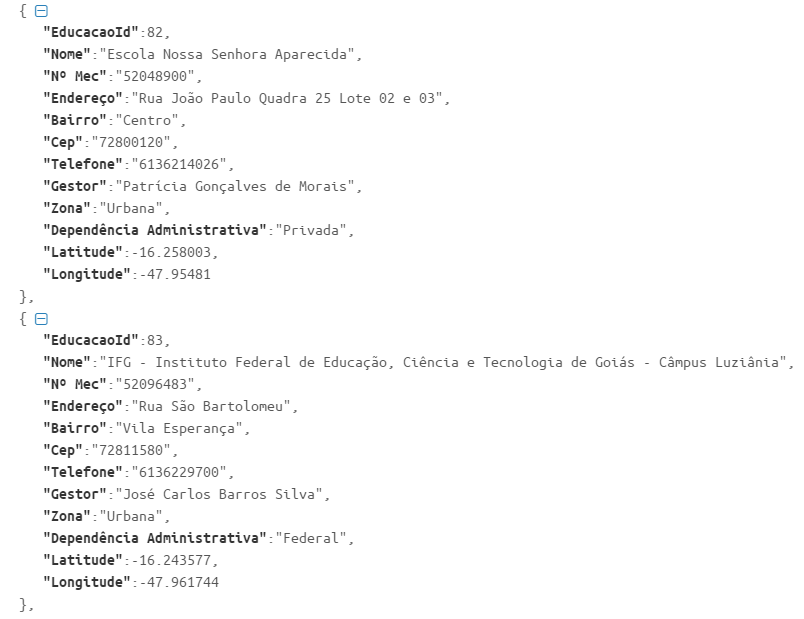
\includegraphics[width=0.75\textwidth]{./img/cap_IV/4-ConsultaJSON}
\caption{Consulta \textit{RESTful} com formato JSON.}
\label{fig:ConsultaJSON}
\end{figure}

A Figura \ref{fig:ConsultaJSON} apresenta o resultado de uma consulta REST no formato JSON. Para realizar chamadas de um serviço \textit{RESTful}, é necessário apenas a passagem de parâmetros (se existirem) através da URL. Por exemplo, pode-se realizar uma consulta das instituições de ensino no SIG Web Luziânia através da URL: \textbf{http://sigluziania/api/mapa/educacao}. Assim, fazendo o uso do mesmo mecanismo usado na utilização de \textit{Web Services}.

\newpage

\section{Interface do SIG Web Luziânia}

O SIG Web Luziânia é composto por duas partes: a georreferenciada (parte inicial) e a área administrativa. Na parte georreferenciada ocorre a visualização dos dados georreferenciados (educação, lazer, saúde e segurança) no mapa. A Figura \ref{fig:PaginaInicial} mostra a página inicial do sistema, composto pela visualização dos dados georreferenciados. Os pontos na cor verde, amarelo, vermelho e azul, representam respectivamente dados sobre educação, lazer saúde e segurança, conforme a legenda apresentada na parte inferior do mapa.

\begin{figure}[h]
\centering
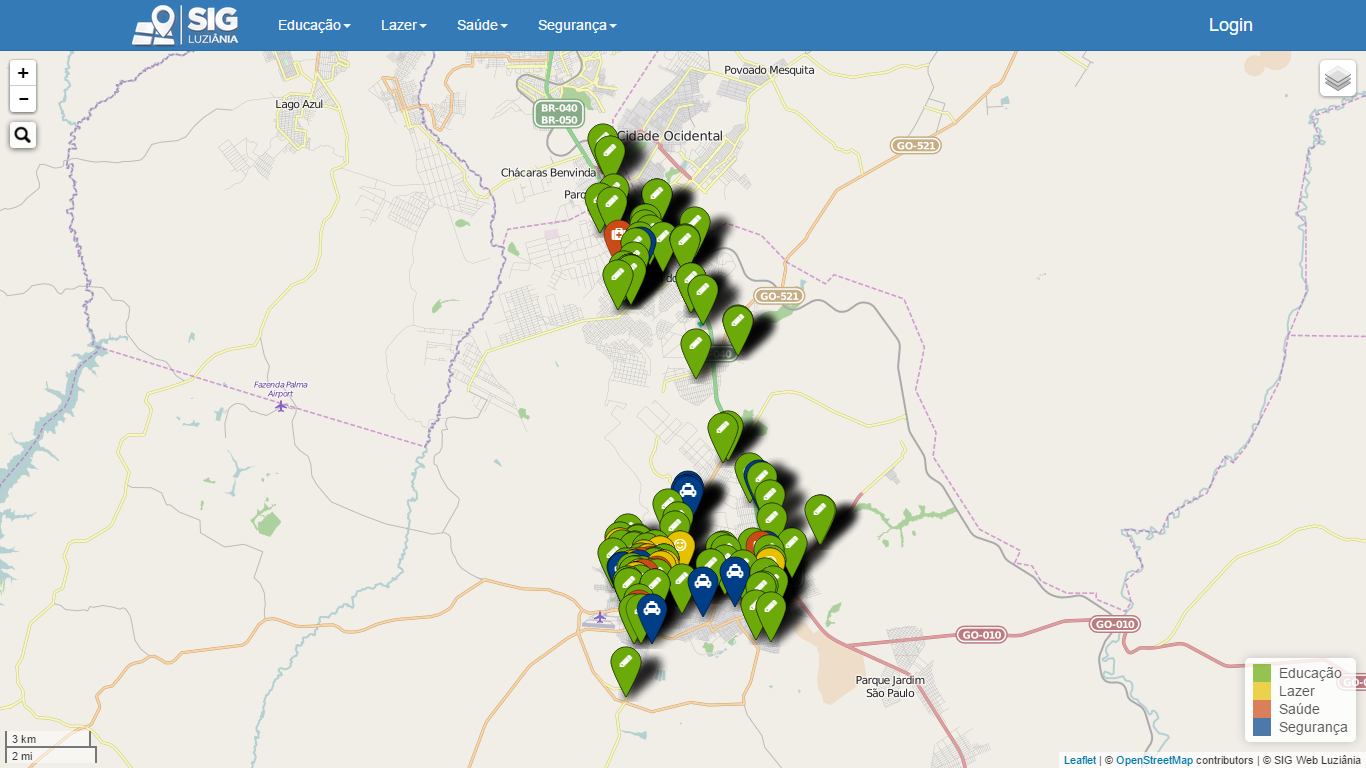
\includegraphics[width=0.80\textwidth]{./img/cap_IV/5-PaginaInicial}
\caption{Página inicial do SIG Web Luziânia.}
\label{fig:PaginaInicial}
\end{figure}

\newpage

Na página inicial do sistema é possível interagir com o mapa. A Figura \ref{fig:BalaoInformacoes} mostra a interação com a visualização dos dados representados no mapa, onde a partir do clique do \textit{mouse} é possível visualizar informações do ponto desejado. A Figura \ref{fig:Camadas} apresenta as camadas representadas no mapa (educação, lazer, saúde e segurança), assim como o tipo de mapa a ser visualizado (rua ou satélite). A Figura \ref{fig:PesquisaMapa} mostra a interação com a parte de pesquisa dos dados do mapa. Ainda é possível interagir com o mapa através do \textit{zoom}.

\begin{figure}[h]
\centering
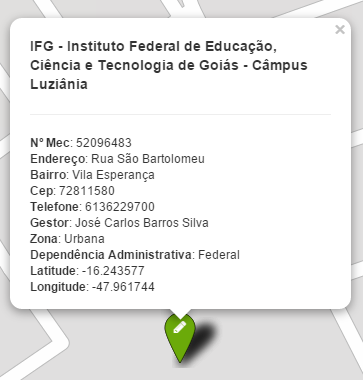
\includegraphics[width=0.36\textwidth]{./img/cap_IV/6-BalaoInformacoes}
\caption{Balão de informações.}
\label{fig:BalaoInformacoes}
\end{figure}

\begin{figure}[h]
\centering
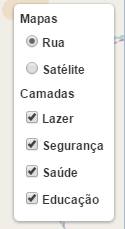
\includegraphics[width=0.14\textwidth]{./img/cap_IV/7-Camadas}
\caption{Camadas do mapa.}
\label{fig:Camadas}
\end{figure}

\begin{figure}[h]
\centering
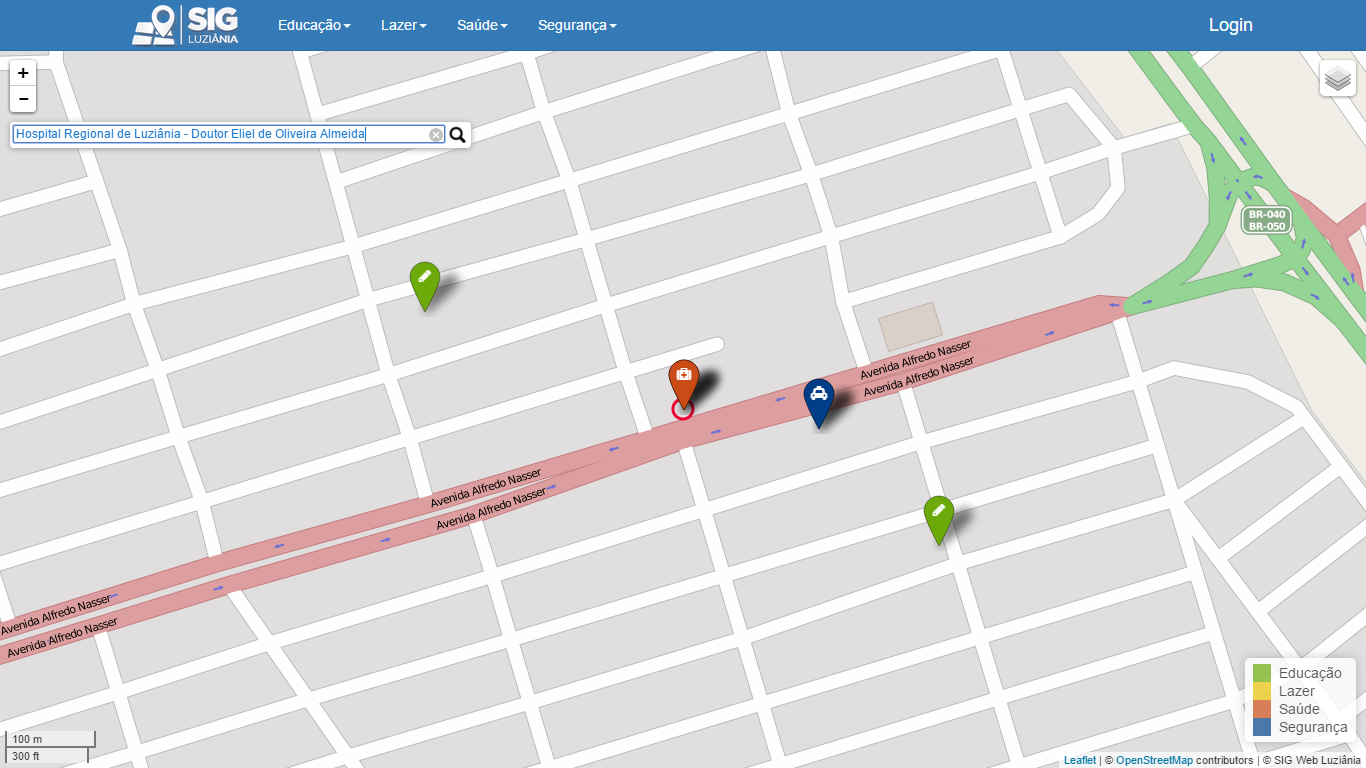
\includegraphics[width=0.80\textwidth]{./img/cap_IV/8-PesquisaMapa}
\caption{Interação com a pesquisa no mapa.}
\label{fig:PesquisaMapa}
\end{figure}

\newpage

Ainda na parte inicial do sistema é apresentado menus onde todos os dados apresentados no mapa são organizados e visualizados. A Figura \ref{fig:Instituicoes} apresenta o menu “Educação”, onde ocorre a visualização dos dados sobre as instituições de ensino, assim como gráficos representando as notas das instituições e suas evoluções no IDEB e ENEM, apresentadas nas Figuras \ref{fig:IDEBInicial}, \ref{fig:IDEBFinal} e \ref{fig:ENEM}.

\begin{figure}[h]
\centering
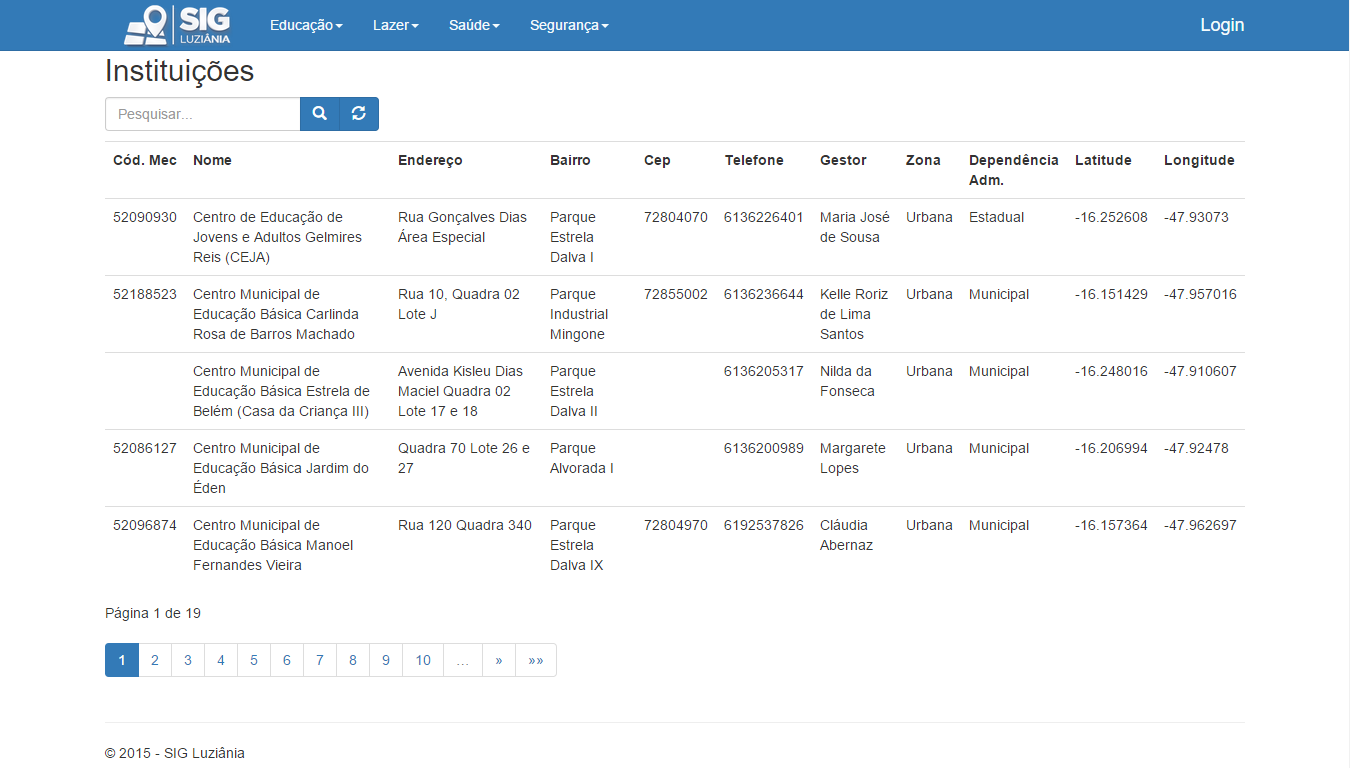
\includegraphics[width=0.80\textwidth]{./img/cap_IV/9-Instituicoes}
\caption{Instituições de ensino.}
\label{fig:Instituicoes}
\end{figure}

\begin{figure}[h]
\centering
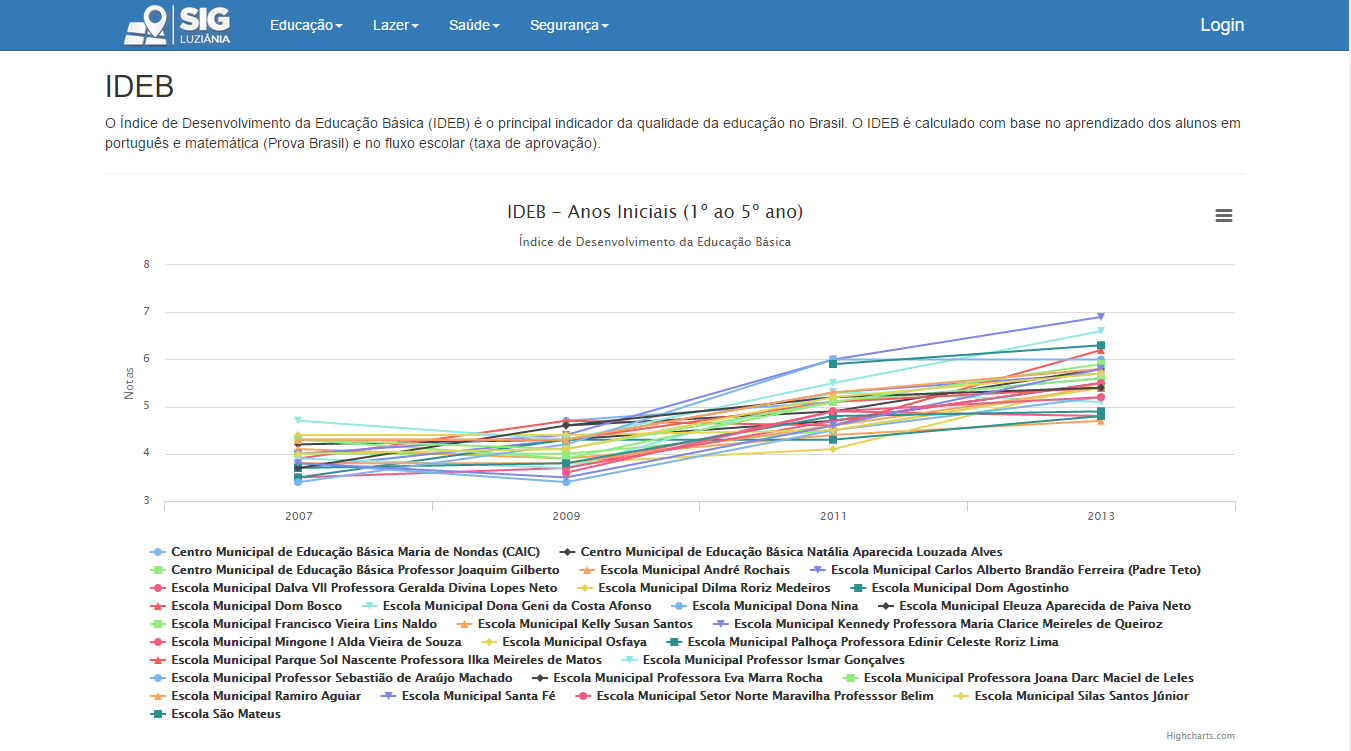
\includegraphics[width=0.80\textwidth]{./img/cap_IV/10-IDEBInicial}
\caption{Notas do IDEB anos iniciais.}
\label{fig:IDEBInicial}
\end{figure}

\newpage

\begin{figure}[h]
\centering
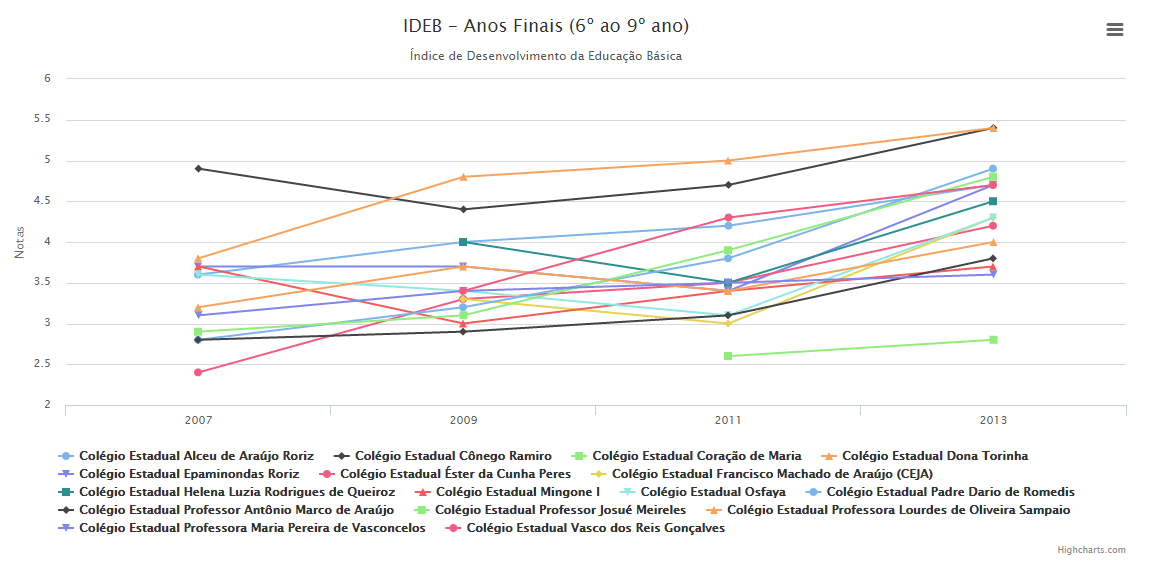
\includegraphics[width=0.80\textwidth]{./img/cap_IV/11-IDEBFinal}
\caption{Notas do IDEB anos finais.}
\label{fig:IDEBFinal}
\end{figure}

\begin{figure}[h]
\centering
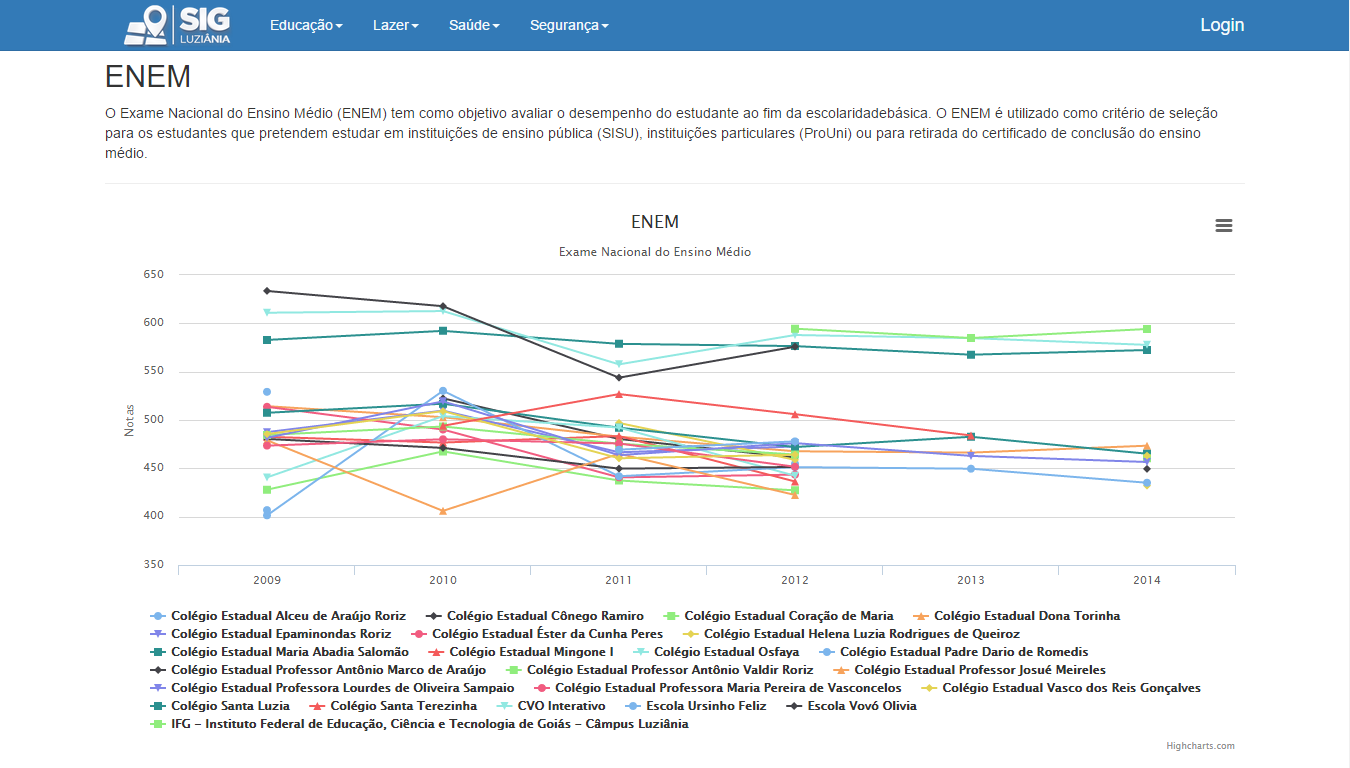
\includegraphics[width=0.80\textwidth]{./img/cap_IV/12-ENEM}
\caption{Notas do ENEM.}
\label{fig:ENEM}
\end{figure}

A Figura \ref{fig:Lazer} é apresentado o menu “Lazer”, contendo as localidades de entretenimento. O menu “Saúde” contém as localidades de saúde, apresentada na Figura \ref{fig:Saude}. A Figura \ref{fig:Especialidade}, apresenta as especialidades presente nas localidades de saúde.

\begin{figure}[h]
\centering
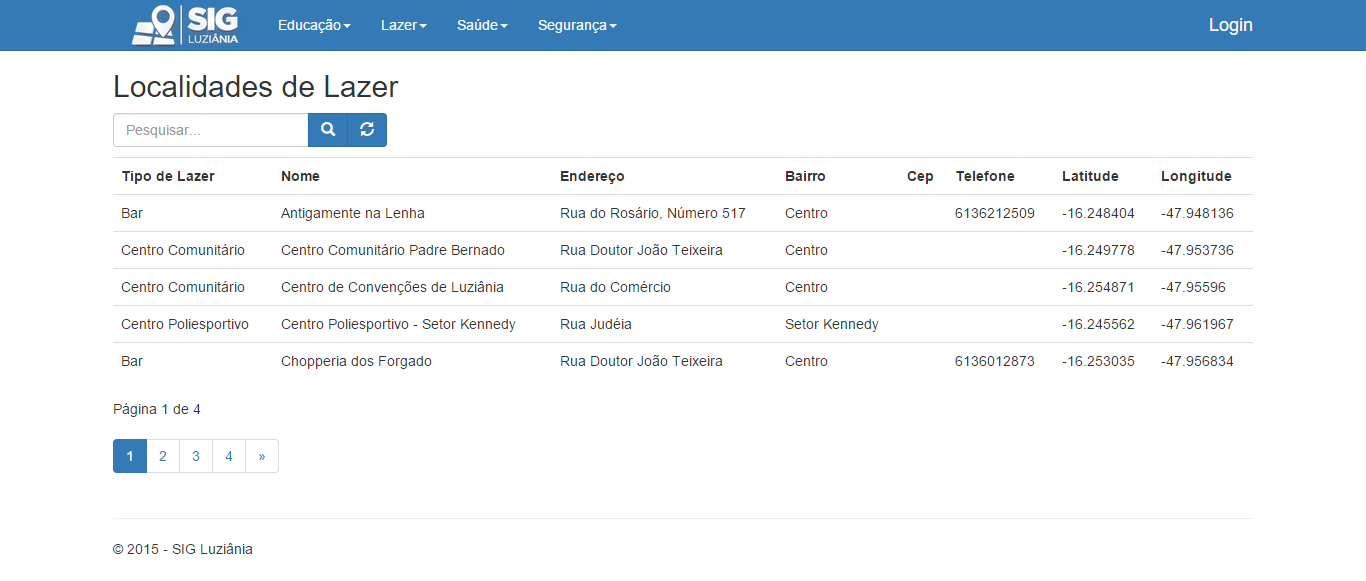
\includegraphics[width=0.80\textwidth]{./img/cap_IV/13-Lazer}
\caption{Localidades de entretenimento.}
\label{fig:Lazer}
\end{figure}

\begin{figure}[h]
\centering
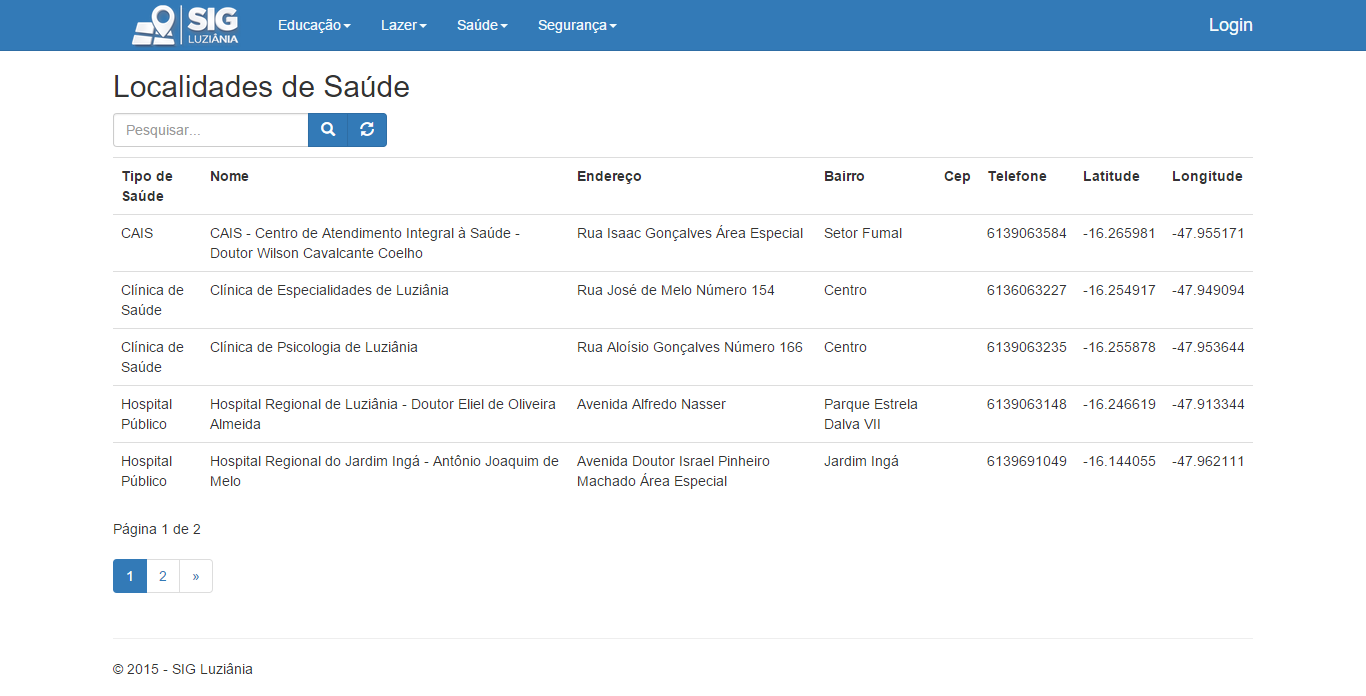
\includegraphics[width=0.80\textwidth]{./img/cap_IV/14-Saude}
\caption{Localidades de saúde.}
\label{fig:Saude}
\end{figure}

\newpage

\begin{figure}[h]
\centering
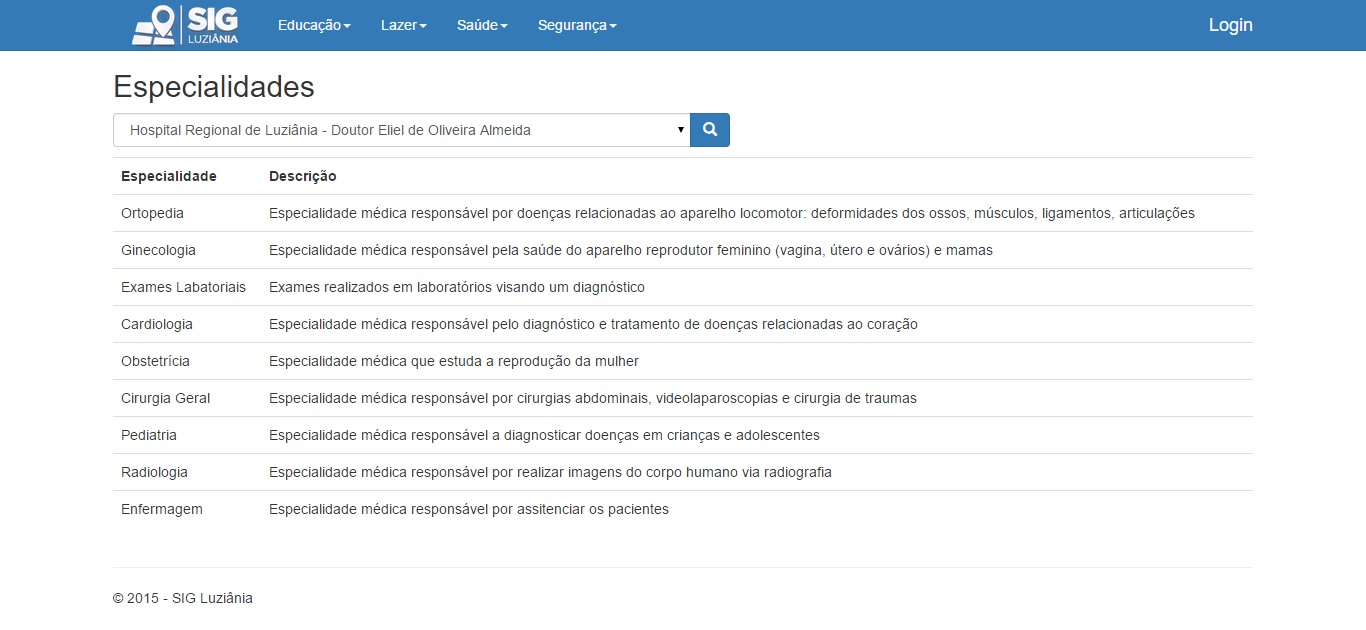
\includegraphics[width=0.80\textwidth]{./img/cap_IV/15-Especialidades}
\caption{Especialidades de saúde.}
\label{fig:Especialidade}
\end{figure}

\newpage

E por fim, no menu “Segurança” é apresentado as localidades de segurança apresentadas na Figura \ref{fig:Seguranca}.

\begin{figure}[h]
\centering
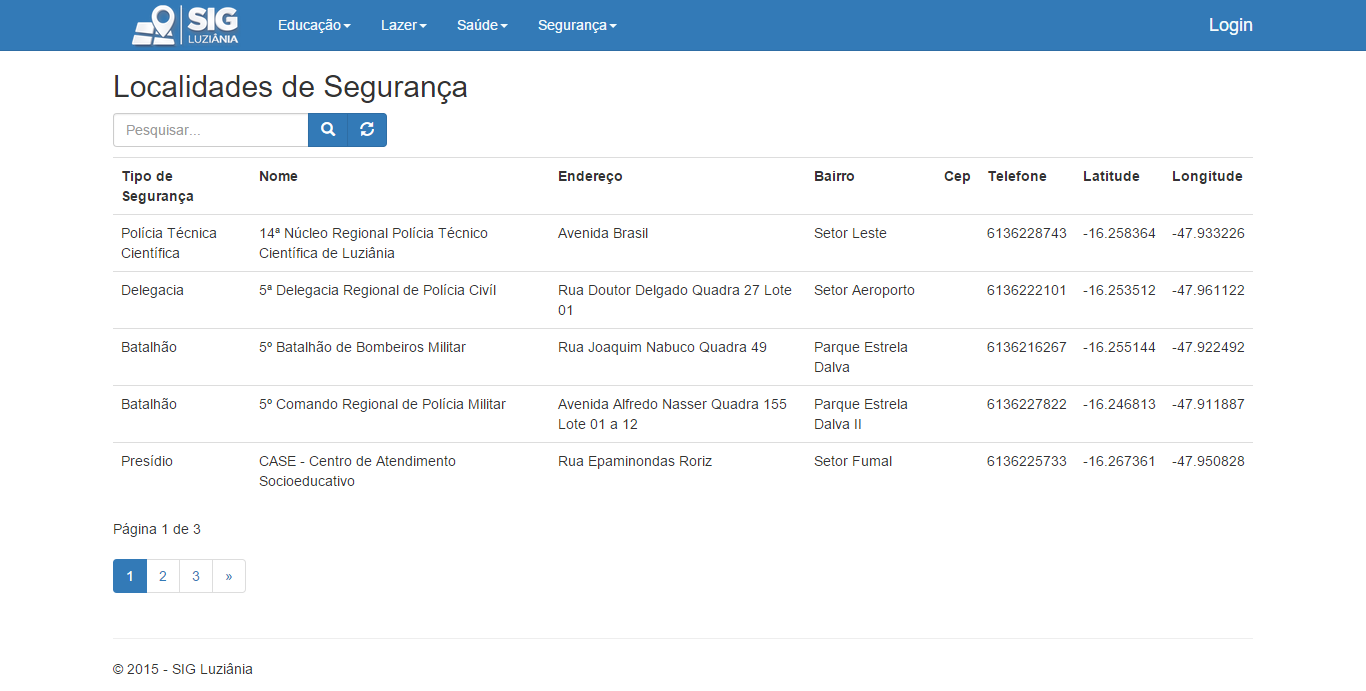
\includegraphics[width=0.80\textwidth]{./img/cap_IV/16-Seguranca}
\caption{Localidades de segurança.}
\label{fig:Seguranca}
\end{figure}

A área administrativa do sistema é responsável pelo acesso e controle dos dados apresentados no mapa. A Figura \ref{fig:Login} exibe a tela de \textit{login} do SIG Web Luziânia para acesso a área administrativa do sistema.

\begin{figure}[h]
\centering
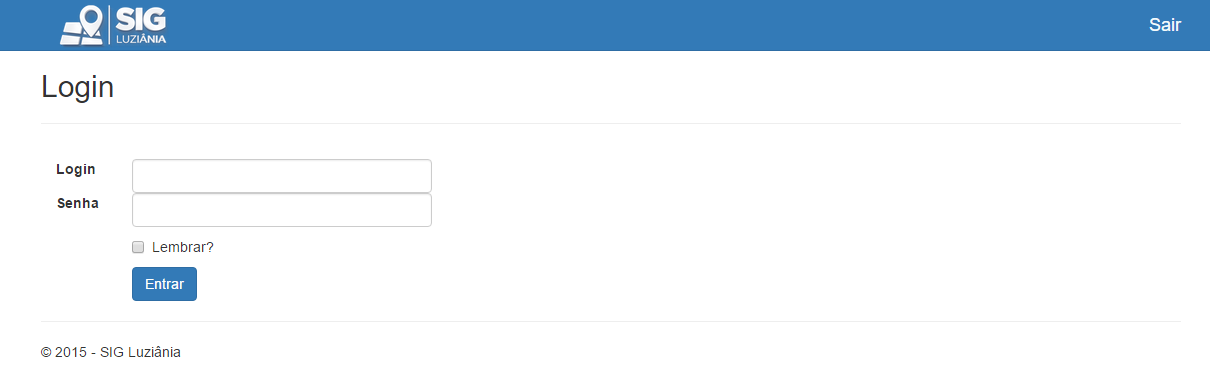
\includegraphics[width=0.80\textwidth]{./img/cap_IV/17-Login}
\caption{Tela de \textit{login}.}
\label{fig:Login}
\end{figure}

Após efetuado o \textit{login} pelo usuário é visualizado a tela da área administrativa, responsável pelo controle dos dados do SIG Web Luziânia, apresentado pela Figura \ref{fig:AreaAdministrativa}.  A área administrativa é composta pelos respectivos menus:

\begin{itemize}
\item “Administrador”: responsável por gerenciar os administradores do sistema;
\item “Educação”: responsável por gerenciar as instituições de ensino e suas avaliações;
\item “Lazer”: responsável por gerenciar as localidades de entretenimento e seus tipos de entretenimento;
\item “Saúde”: responsável por gerenciar as localidades de saúde, tipos de localidades e especialidades;
\item “Segurança”: responsável por gerenciar todas as localidades de segurança e seus tipos de localidades.
\end{itemize}

\newpage

\begin{figure}[h]
\centering
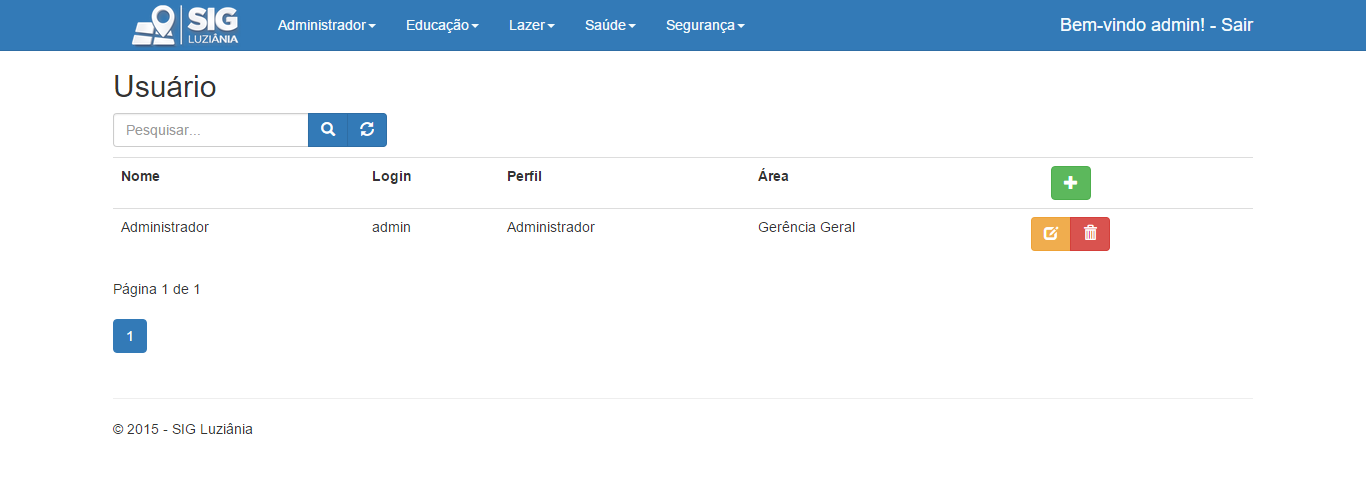
\includegraphics[width=0.80\textwidth]{./img/cap_IV/18-AreaAdministrativa}
\caption{Área administrativa do sistema.}
\label{fig:AreaAdministrativa}
\end{figure}

As Figuras \ref{fig:AdmEducacao}, \ref{fig:AdmLazer}, \ref{fig:AdmSaude} e \ref{fig:AdmSeguranca} apresentam a área de controle de dados dos menus: “Educação”, “Lazer”, “Saúde” e “Segurança”.

\begin{figure}[h]
\centering
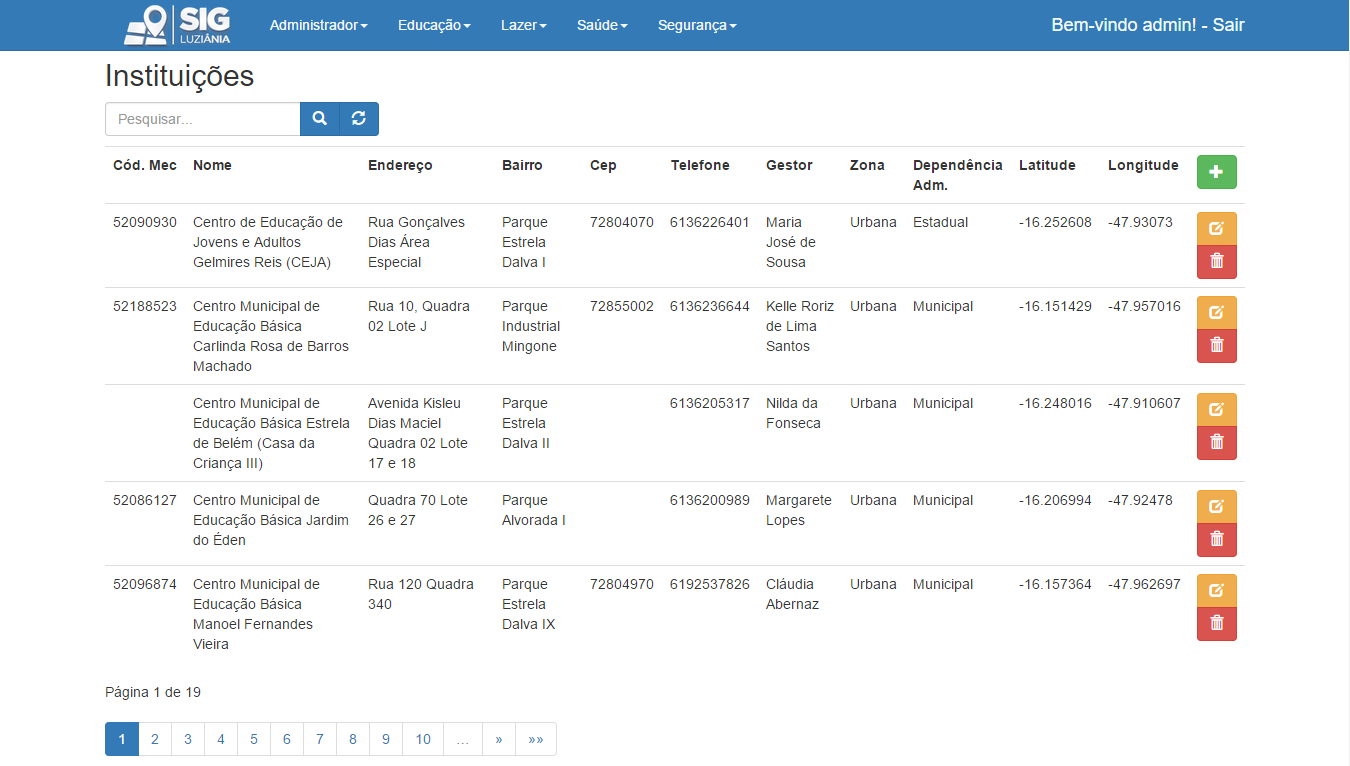
\includegraphics[width=0.80\textwidth]{./img/cap_IV/19-AdmEducacao}
\caption{Área administrativa dos dados de educação.}
\label{fig:AdmEducacao}
\end{figure}

\begin{figure}[h]
\centering
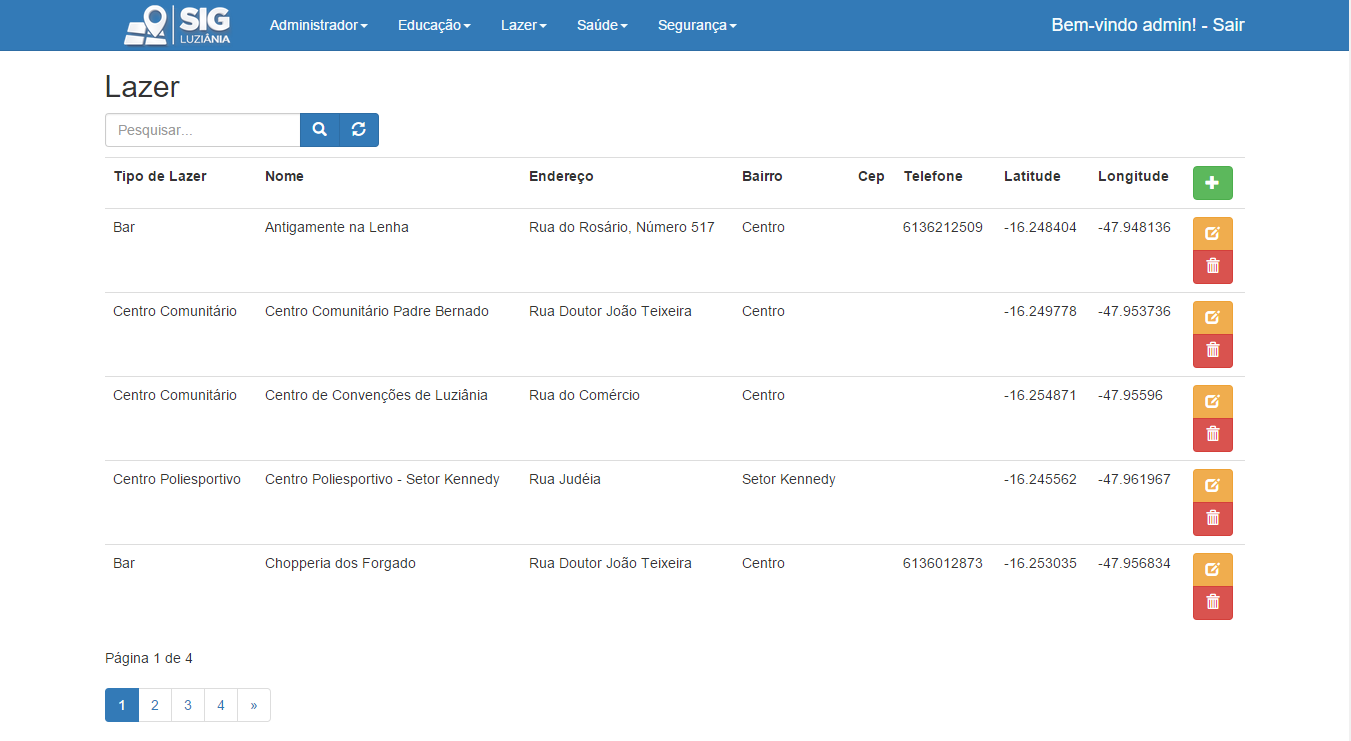
\includegraphics[width=0.80\textwidth]{./img/cap_IV/20-AdmLazer}
\caption{Área administrativa dos dados de entretenimento.}
\label{fig:AdmLazer}
\end{figure}

\newpage

\begin{figure}[h]
\centering
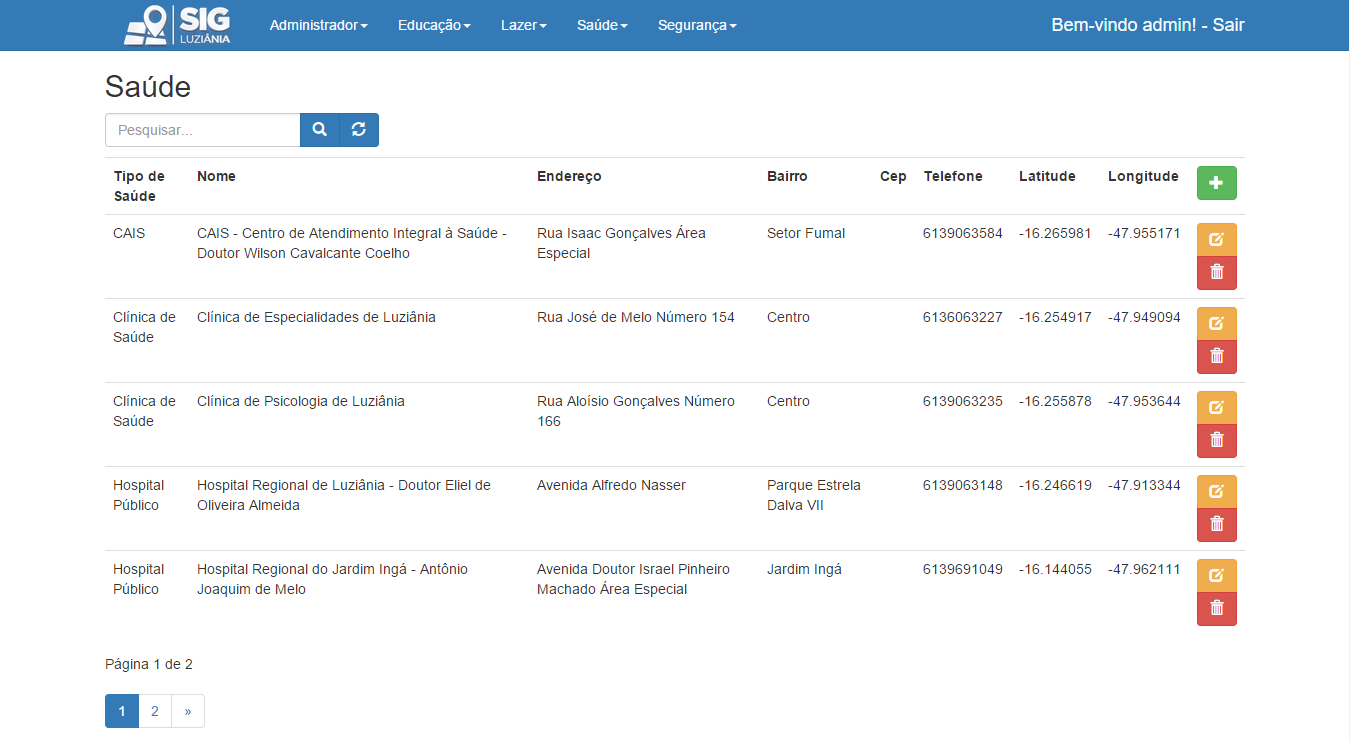
\includegraphics[width=0.80\textwidth]{./img/cap_IV/21-AdmSaude}
\caption{Área administrativa dos dados de saúde.}
\label{fig:AdmSaude}
\end{figure}

\begin{figure}[h]
\centering
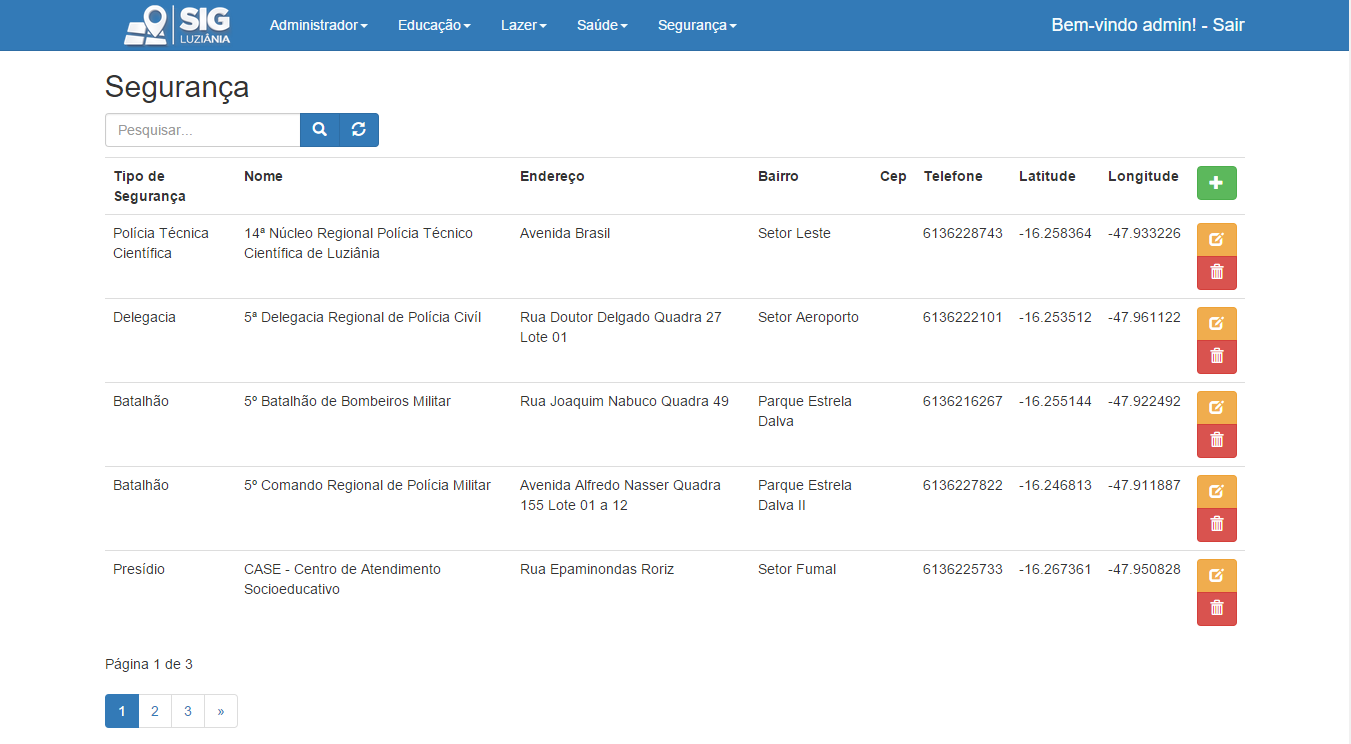
\includegraphics[width=0.80\textwidth]{./img/cap_IV/22-AdmSeguranca}
\caption{Área administrativa dos dados de segurança.}
\label{fig:AdmSeguranca}
\end{figure}

\newpage

As Figuras \ref{fig:AdmAvaliacao} e \ref{fig:AdmEspecialidade} apresentam os controles de dados das avaliações e especialidades presentes respectivamente nos menus de "Educação" e "Saúde". Nessa área do sistema é realizado o vínculo das avaliações com as instituições de ensino e as especialidades com as instituições de saúde.

\begin{figure}[h]
\centering
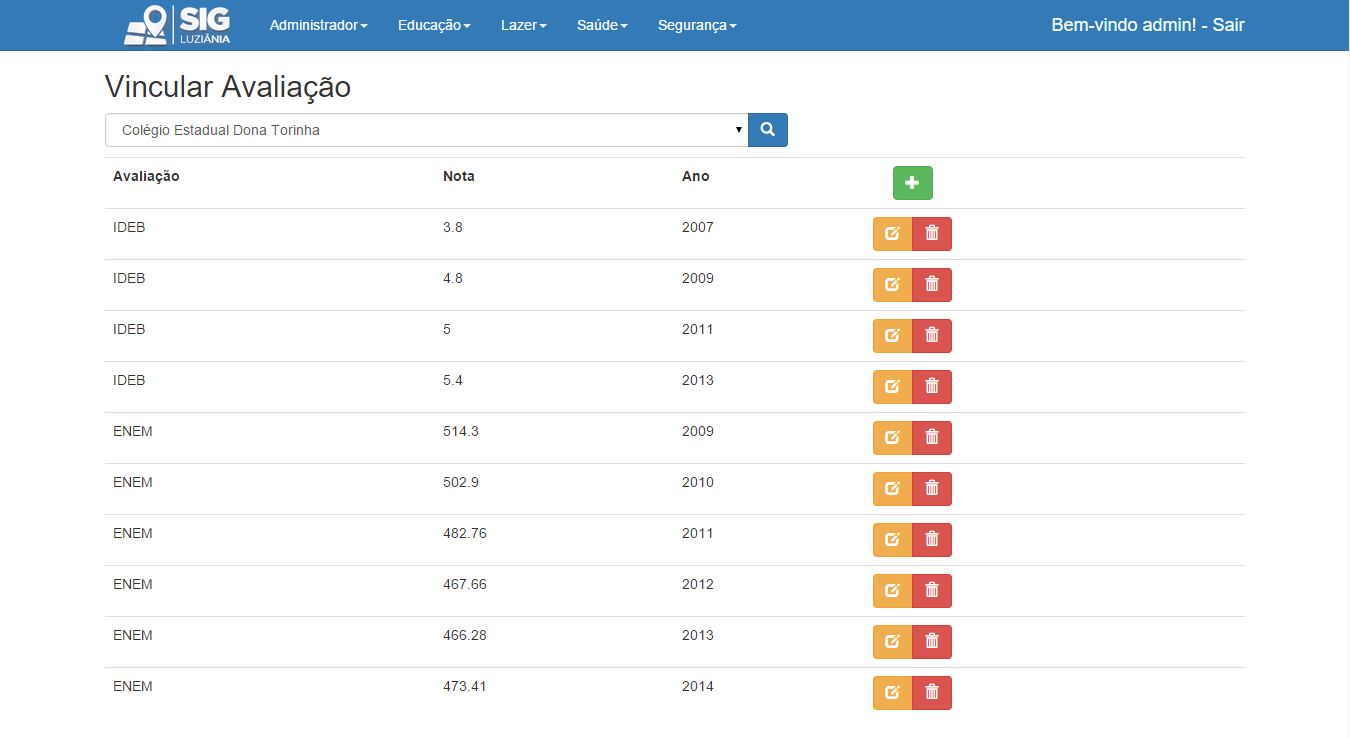
\includegraphics[width=0.80\textwidth]{./img/cap_IV/23-AdmAvaliacao}
\caption{Área administrativa de avaliações.}
\label{fig:AdmAvaliacao}
\end{figure}

\newpage

\begin{figure}[h]
\centering
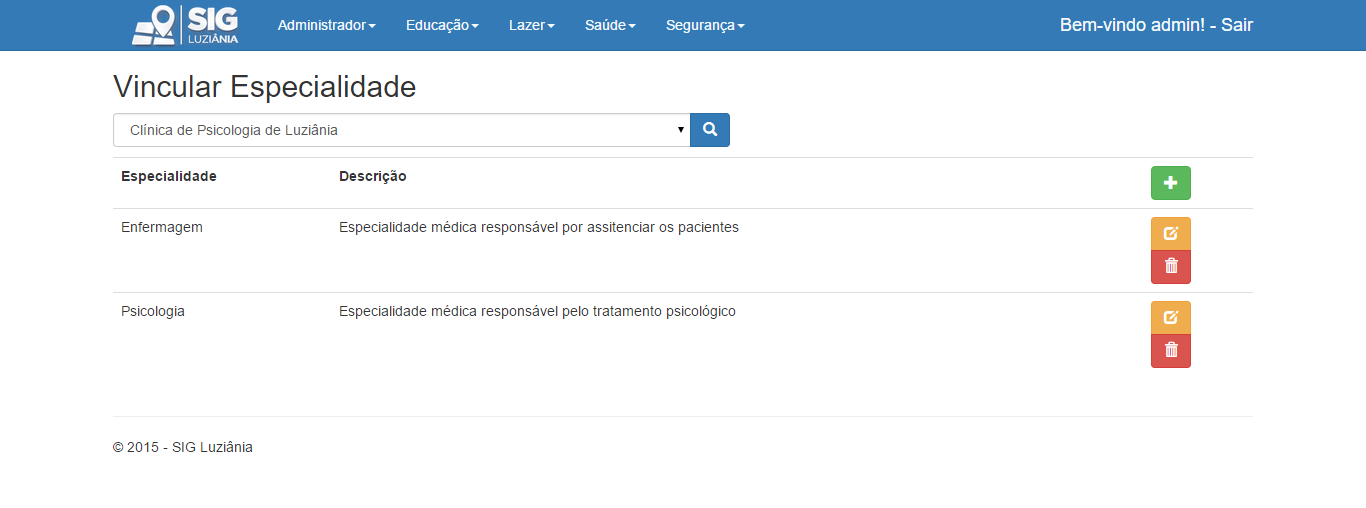
\includegraphics[width=0.80\textwidth]{./img/cap_IV/24-AdmEspecialidade}
\caption{Área administrativa de especialidades.}
\label{fig:AdmEspecialidade}
\end{figure}

Em toda a área administrativa do sistema, é realizado todas as operações de controle de dados (inserir, visualizar, atualizar e excluir). As operações de inserir, atualizar e excluir estão presentes em \textit{pop-up’s} presente em todos os menus do sistema. A Figura \ref{fig:AdmAdicionar}, \ref{fig:AdmEditar} e \ref{fig:AdmExcluir} representam respectivamente cada uma das operações no menu “Saúde”.

\begin{figure}[h]
\centering
\includegraphics[width=0.80\textwidth]{./img/cap_IV/25-AdmAdicionar}
\caption{\textit{Pop-up} para adicionar localidade de saúde.}
\label{fig:AdmAdicionar}
\end{figure}

\newpage

\begin{figure}[h]
\centering
\includegraphics[width=0.80\textwidth]{./img/cap_IV/26-AdmEditar}
\caption{\textit{Pop-up} para editar localidade de saúde.}
\label{fig:AdmEditar}
\end{figure}

\begin{figure}[h]
\centering
\includegraphics[width=0.80\textwidth]{./img/cap_IV/27-AdmExcluir}
\caption{\textit{Pop-up} para excluir localidade de saúde.}
\label{fig:AdmExcluir}
\end{figure}

O SIG Web Luziânia foi construído utilizando as tecnologias Web mais recentes como o HTML5, \textit{Cascading Style Sheets 3} (CSS3) e Javascript. Por esse motivo, o sistema é totalmente responsível e acessível em dispositivos móveis. A Figura \ref{fig:MobileMapa} e a Figura \ref{fig:MobileAdm} apresentam essa acessibilidade.

\begin{figure}[h]
\centering
\includegraphics[width=0.80\textwidth]{./img/cap_IV/28-MobileMapa}
\caption{Visualização da página inicial do sistema em um \textit{Smartphone}.}
\label{fig:MobileMapa}
\end{figure}

\newpage

\begin{figure}[h]
\centering
\includegraphics[width=0.80\textwidth]{./img/cap_IV/29-MobileAdm}
\caption{Visualização da área administrativa do sistema em um \textit{Smartphone}.}
\label{fig:MobileAdm}
\end{figure}

\section{Trabalhos Relacionados}

A grande extensão do território brasileiro em conjunto com sua população, torna o uso de um SIG para o gerenciamento das informações fundamental, seja no âmbito municipal, estadual e federal. Grandes cidades brasileiras possuem SIGs Web para o gerenciamento e visualização das informações de uma maneira pública a população.

Como SIGs Web relacionados a este trabalho temos: Sistema de Informação Geográfica de Goiânia (SIGGO), Sistema de Informação Geográfica da Bahia (SIG Bahia) e o Sistema Municipal de Informações Urbanas (SIURB).

\newpage

O SIGGO \cite{siggo} apresenta informações da cidade de Goiânia, a Figura \ref{fig:SIGGO} apresenta a página inicial do sistema. Através do SIGGO é possível obter as seguintes informações:

\begin{itemize}
\item Bairros, quadras e lotes;
\item Ruas, praças e avenidas;
\item Hidrografia;
\item Escolas;
\item Unidades de saúde.
\end{itemize}

\begin{figure}[h]
\centering
\includegraphics[width=0.80\textwidth]{./img/cap_IV/30-SIGGO}
\caption{Página inicial do SIGGO.}
\label{fig:SIGGO}
\end{figure}

O SIG Bahia \cite{sigbahia} apresenta informações do estado da Bahia, a Figura \ref{fig:SIGBahia} apresenta a página inicial do sistema. O SIG Bahia apresenta um grande número de informações disponíveis, as principais são:

\begin{itemize}
\item Hidrografia;
\item Sistema de transporte;
\item Rodoviais, estradas, ferroviais;
\item Biodiversidade;
\item Unidades de conservações;
\item Mapas sociais;
\item Mapas geológicos.
\end{itemize}

\newpage

\begin{figure}[h]
\centering
\includegraphics[width=0.80\textwidth]{./img/cap_IV/31-SIGBahia}
\caption{Página inicial SIG Bahia.}
\label{fig:SIGBahia}
\end{figure}

Por fim, o SIURB \cite{siurg} é utilizado na tomada de decisão da administração municipal do município do Rio de Janeiro. A Figura \ref{fig:SIURB} apresenta a página inicial do SIURB.

\begin{figure}[h]
\centering
\includegraphics[width=0.80\textwidth]{./img/cap_IV/32-SIURB}
\caption{Página inicial do SIURB.}
\label{fig:SIURB}
\end{figure}

As principais informações disponíveis no sistema são:

\begin{itemize}
\item Ações da prefeitura nas áreas pacificadas;
\item Segurança;
\item Transporte público;
\item Saúde;
\item Educação;
\item Lazer e cultura.
\end{itemize}

A principal característica presente nos SIGs Web citados e no SIG Web Luziânia é tornar a tomada de decisão mais ágil e precisa para os gestores que utilizam o sistema. A grande diferença é a utilização da tecnologia \textit{Adobe Flex} na interface no sistema. Essa tecnologia impossibilita que o sistema seja responsível em dispositivos móveis, tornando a interface pouco amigável ao usuário. O uso de tecnologias como HTML5, CSS3 e Javascript se faz essencial para que o SIG Web esteja disponível em dispositivos móveis, como ocorre no SIG Web Luziânia.
\chapter{Conclusão}
\label{cap:conclusao}

A cidade de Luziânia possui atualmente um grande volume de informações relacionadas a serviços básicos a população, compostos pelos serviços de: educação, lazer, saúde e segurança. Todas as informações são organizadas em documentos físicos e planilhas eletrônicas, dificultando o acesso posterior e ocasionando possíveis inconsistências no armazenamento e na recuperação dessas informações. Para resolver esse problema, foram propostos as seguintes soluções: a criação de um banco de dados geográfico para armazenamento dos dados que possuam localização geográfica e a criação de um sistema de informação geográfico para organização e apresentação dos dados de forma georreferenciada.

Primeiramente, foi realizado o processo de coleta e organização das informações, sendo posteriomente adicionadas ao banco de dados. Em seguida, começou a implementação de um SIG Web. Todo o processo de implementação do sistema fez uso de ferramentas livres para criação.

Em cumprimento dos objetivos deste trabalho, foi desenvolvido o SIG Web Luziânia com o objetivo de organizar, gerenciar e visualizar dados relacionados aos serviços de educação, lazer, saúde e segurança. O padrão OMT-G foi utilizado na criação do modelo de dados, a extensão espacial utilizada no banco de dados geográfico foi o PostGIS, e por fim, as principais tecnologias utilizadas no desenvolvimento do SIG Web Luziânia foram: C\#, \textit{ASP.NET MVC}, HTML5, Javascript e o \textit{Leaflet}.

Como vantagens e benefícios para a cidade de Luziânia, o SIG Web Luziânia apresenta as seguintes perspectivas:

\begin{itemize}
\item Organiza as informações evitando inconsistência;
\item Facilita o gerenciamento das informações pelos órgãos competentes;
\item Transparência das informações para a população de Luziânia; 
\item Apresenta os dados de forma georreferenciada;
\item Possibilita a criação de novas funcionalidades e serviços;
\item Possibilita o acesso as informações em dispositivos móveis e \textit{desktops} a partir do \textit{browser}.
\end{itemize}

Como trabalhos futuros, pretende-se ter o cadastro de mais informações, a criação de novos serviços, disponibilização dos dados do sistema para \textit{download} e publicação do sistema na Internet.

% ----------------------------------------------------------
% Finaliza a parte no bookmark do PDF
% para que se inicie o bookmark na raiz
% e adiciona espaço de parte no Sumário
% ----------------------------------------------------------
\phantompart


% ----------------------------------------------------------
% ELEMENTOS PÓS-TEXTUAIS
% ----------------------------------------------------------
\postextual
% ----------------------------------------------------------

% ----------------------------------------------------------
% Referências bibliográficas
% ----------------------------------------------------------
\bibliography{bib/bib}

% ----------------------------------------------------------
% Glossário
% ----------------------------------------------------------
%
% Consulte o manual da classe abntex2 para orientações sobre o glossário.
%
%\glossary

% ----------------------------------------------------------
% Apêndices
% ----------------------------------------------------------

% ---
% Inicia os apêndices
% ---
%\begin{apendicesenv}
%
%% Imprime uma página indicando o início dos apêndices
%\partapendices
%
%% ----------------------------------------------------------
%\chapter{Quisque libero justo}
%% ----------------------------------------------------------
%
%\lipsum[50]
%
%% ----------------------------------------------------------
%\chapter{Nullam elementum urna vel imperdiet sodales elit ipsum pharetra ligula
%ac pretium ante justo a nulla curabitur tristique arcu eu metus}
%% ----------------------------------------------------------
%\lipsum[55-57]
%
%\end{apendicesenv}
% ---


% ----------------------------------------------------------
% Anexos
% ----------------------------------------------------------

% ---
% Inicia os anexos
% ---
%\begin{anexosenv}
%
%% Imprime uma página indicando o início dos anexos
%\partanexos
%
%\end{anexosenv}

%---------------------------------------------------------------------
% INDICE REMISSIVO
%---------------------------------------------------------------------
\phantompart
\printindex
%---------------------------------------------------------------------

\end{document}